% **************************************************************************************************************
% A Classic Thesis Style
% An Homage to The Elements of Typographic Style
%
% Copyright (C) 2012 Andr\'e Miede http://www.miede.de
%
% If you like the style then I would appreciate a postcard. My address 
% can be found in the file ClassicThesis.pdf. A collection of the 
% postcards I received so far is available online at 
% http://postcards.miede.de
%
% License:
% This program is free software; you can redistribute it and/or modify
% it under the terms of the GNU General Public License as published by
% the Free Software Foundation; either version 2 of the License, or
% (at your option) any later version.
%
% This program is distributed in the hope that it will be useful,
% but WITHOUT ANY WARRANTY; without even the implied warranty of
% MERCHANTABILITY or FITNESS FOR A PARTICULAR PURPOSE.  See the
% GNU General Public License for more details.
%
% You should have received a copy of the GNU General Public License
% along with this program; see the file COPYING.  If not, write to
% the Free Software Foundation, Inc., 59 Temple Place - Suite 330,
% Boston, MA 02111-1307, USA.
%
% **************************************************************************************************************
% Note:
%    * You must not use "u etc. in strings/commands that will be spaced out (use \"u or real umlauts instead)
%    * New enumeration (small caps): \begin{aenumerate} \end{aenumerate}
%    * For margin notes: \marginpar or \graffito{}
%    * Do not use bold fonts in this style, it is designed around them
%    * Use tables as in the examples
%    * See classicthesis-preamble.sty for useful commands
% **************************************************************************************************************
% To Do:
%		 * [high] Check this out: http://www.golatex.de/koma-script-warnung-in-verbindung-mit-listings-package-t2058.html
%    * [medium] mathbb in section-titles/chapter-titles => disappears somehow in headlines!!!
% **************************************************************************************************************
\documentclass[ twoside,openright,titlepage,numbers=noenddot,headinclude,%1headlines,% letterpaper a4paper
                footinclude=true,cleardoublepage=empty,abstractoff, % <--- obsolete, remove (todo)
                BCOR=5mm,paper=a4,fontsize=11pt,%11pt,a4paper,%
                british,openany%
                ]{scrreprt}

%********************************************************************
% Note: Make all your adjustments in here
%*******************************************************
% ****************************************************************************************************
% classicthesis-config.tex 
% formerly known as loadpackages.sty, classicthesis-ldpkg.sty, and classicthesis-preamble.sty 
% Use it at the beginning of your ClassicThesis.tex, or as a LaTeX Preamble 
% in your ClassicThesis.{tex,lyx} with % ****************************************************************************************************
% classicthesis-config.tex 
% formerly known as loadpackages.sty, classicthesis-ldpkg.sty, and classicthesis-preamble.sty 
% Use it at the beginning of your ClassicThesis.tex, or as a LaTeX Preamble 
% in your ClassicThesis.{tex,lyx} with % ****************************************************************************************************
% classicthesis-config.tex 
% formerly known as loadpackages.sty, classicthesis-ldpkg.sty, and classicthesis-preamble.sty 
% Use it at the beginning of your ClassicThesis.tex, or as a LaTeX Preamble 
% in your ClassicThesis.{tex,lyx} with \input{classicthesis-config}
% ****************************************************************************************************  
% If you like the classicthesis, then I would appreciate a postcard. 
% My address can be found in the file ClassicThesis.pdf. A collection 
% of the postcards I received so far is available online at 
% http://postcards.miede.de
% ****************************************************************************************************

% ****************************************************************************************************
% 1. Configure classicthesis for your needs here, e.g., remove "drafting" below 
% in order to deactivate the time-stamp on the pages
% ****************************************************************************************************
\PassOptionsToPackage{eulerchapternumbers,listings, %drafting,%
				 pdfspacing,%floatperchapter,%linedheaders,%
				 subfig,beramono,eulermath,parts}{classicthesis}										
% ********************************************************************
% Available options for classicthesis.sty 
% (see ClassicThesis.pdf for more information):
% drafting
% parts nochapters linedheaders
% eulerchapternumbers beramono eulermath pdfspacing minionprospacing
% tocaligned dottedtoc manychapters
% listings floatperchapter subfig
% ********************************************************************

% ********************************************************************
% Triggers for this config
% ******************************************************************** 
\usepackage{ifthen}
\newboolean{enable-backrefs} % enable backrefs in the bibliography
\setboolean{enable-backrefs}{false} % true false
% ****************************************************************************************************


% ****************************************************************************************************
% 2. Personal data and user ad-hoc commands
% ****************************************************************************************************
\newcommand{\myTitle}{Scaling Learning to Rank to Big Data\xspace}
\newcommand{\mySubtitle}{A study concerning parallelisation of Learning to Rank algorithms using the MapReduce computing model\xspace}
\newcommand{\myDegree}{Bsc.\xspace}
\newcommand{\myName}{Niek Tax\xspace}
\newcommand{\myProf}{Dr. ir. Djoerd Hiemstra\xspace}
\newcommand{\mySupervisor}{Sander Bockting\xspace}
\newcommand{\myFaculty}{Faculty of Electrical Engineering, Mathematics and Computer Science (EEMCS)\xspace}
\newcommand{\myDepartment}{Research Chair Databases\xspace}
\newcommand{\myUni}{University of Twente\xspace}
\newcommand{\myLocation}{Enschede\xspace}
\newcommand{\myTime}{Februari 2014\xspace}
\newcommand{\myVersion}{version 0.1\xspace}

% ********************************************************************
% Setup, finetuning, and useful commands
% ********************************************************************
\newcounter{dummy} % necessary for correct hyperlinks (to index, bib, etc.)
\newlength{\abcd} % for ab..z string length calculation
\providecommand{\mLyX}{L\kern-.1667em\lower.25em\hbox{Y}\kern-.125emX\@}
\newcommand{\ie}{i.\,e.}
\newcommand{\Ie}{I.\,e.}
\newcommand{\eg}{e.\,g.}
\newcommand{\Eg}{E.\,g.} 
% ****************************************************************************************************


% ****************************************************************************************************
% 3. Loading some handy packages
% ****************************************************************************************************
% ******************************************************************** 
% Packages with options that might require adjustments
% ******************************************************************** 
\PassOptionsToPackage{latin9}{inputenc}	% latin9 (ISO-8859-9) = latin1+"Euro sign"
 \usepackage{inputenc}				

%\PassOptionsToPackage{ngerman,american}{babel}   % change this to your language(s)
% Spanish languages need extra options in order to work with this template
%\PassOptionsToPackage{spanish,es-lcroman}{babel}
 \usepackage{babel}					

\PassOptionsToPackage{fleqn}{amsmath}		% math environments and more by the AMS 
 \usepackage{amsmath}

% ******************************************************************** 
% General useful packages
% ******************************************************************** 
\PassOptionsToPackage{T1}{fontenc} % T2A for cyrillics
	\usepackage{fontenc}     
\usepackage{textcomp} % fix warning with missing font shapes
\usepackage{scrhack} % fix warnings when using KOMA with listings package          
\usepackage{xspace} % to get the spacing after macros right
\usepackage{mparhack} % get marginpar right
\usepackage{newclude}
\usepackage[]{algorithm2e}
\usepackage{mathrsfs}
\usepackage{booktabs}
\usepackage{array}
\usepackage{longtable}
\usepackage{fixltx2e} % fixes some LaTeX stuff
\usepackage{notes}
\usepackage{watermark}
\PassOptionsToPackage{printonlyused,smaller}{acronym}
	\usepackage{acronym} % nice macros for handling all acronyms in the thesis
%\renewcommand*{\acsfont}[1]{\textssc{#1}} % for MinionPro
\renewcommand{\bflabel}[1]{{#1}\hfill} % fix the list of acronyms
% ****************************************************************************************************


% ****************************************************************************************************
% 4. Setup floats: tables, (sub)figures, and captions
% ****************************************************************************************************
\usepackage{tabularx} % better tables
	\setlength{\extrarowheight}{3pt} % increase table row height
\newcommand{\tableheadline}[1]{\multicolumn{1}{c}{\spacedlowsmallcaps{#1}}}
\newcommand{\myfloatalign}{\centering} % to be used with each float for alignment
\usepackage{caption}
\captionsetup{format=hang,font=small}
\usepackage{subfig}  
% ****************************************************************************************************


% ****************************************************************************************************
% 5. Setup code listings
% ****************************************************************************************************
\usepackage{listings} 
%\lstset{emph={trueIndex,root},emphstyle=\color{BlueViolet}}%\underbar} % for special keywords
\lstset{language=[LaTeX]Tex,%C++,
    keywordstyle=\color{RoyalBlue},%\bfseries,
    basicstyle=\small\ttfamily,
    %identifierstyle=\color{NavyBlue},
    commentstyle=\color{Green}\ttfamily,
    stringstyle=\rmfamily,
    numbers=none,%left,%
    numberstyle=\scriptsize,%\tiny
    stepnumber=5,
    numbersep=8pt,
    showstringspaces=false,
    breaklines=true,
    frameround=ftff,
    frame=single,
    belowcaptionskip=.75\baselineskip
    %frame=L
} 
% ****************************************************************************************************
% 6. PDFLaTeX, hyperreferences and citation backreferences
% ****************************************************************************************************
% ********************************************************************
% Using PDFLaTeX
% ********************************************************************
\PassOptionsToPackage{pdftex,hyperfootnotes=false,pdfpagelabels}{hyperref}
	\usepackage{hyperref}  % backref linktocpage pagebackref
\pdfcompresslevel=9
\pdfadjustspacing=1 
\PassOptionsToPackage{pdftex}{graphicx}
	\usepackage{graphicx} 

% ********************************************************************
% Setup the style of the backrefs from the bibliography
% (translate the options to any language you use)
% ********************************************************************
\newcommand{\backrefnotcitedstring}{\relax}%(Not cited.)
\newcommand{\backrefcitedsinglestring}[1]{(Cited on page~#1.)}
\newcommand{\backrefcitedmultistring}[1]{(Cited on pages~#1.)}
\ifthenelse{\boolean{enable-backrefs}}%
{%
		\PassOptionsToPackage{hyperpageref}{backref}
		\usepackage{backref} % to be loaded after hyperref package 
		   \renewcommand{\backreftwosep}{ and~} % separate 2 pages
		   \renewcommand{\backreflastsep}{, and~} % separate last of longer list
		   \renewcommand*{\backref}[1]{}  % disable standard
		   \renewcommand*{\backrefalt}[4]{% detailed backref
		      \ifcase #1 %
		         \backrefnotcitedstring%
		      \or%
		         \backrefcitedsinglestring{#2}%
		      \else%
		         \backrefcitedmultistring{#2}%
		      \fi}%
}{\relax}    

% ********************************************************************
% Hyperreferences
% ********************************************************************
\hypersetup{%
    %draft,	% = no hyperlinking at all (useful in b/w printouts)
    colorlinks=true, linktocpage=true, pdfstartpage=3, pdfstartview=FitV,%
    % uncomment the following line if you want to have black links (e.g., for printing)
    %colorlinks=false, linktocpage=false, pdfborder={0 0 0}, pdfstartpage=3, pdfstartview=FitV,% 
    breaklinks=true, pdfpagemode=UseNone, pageanchor=true, pdfpagemode=UseOutlines,%
    plainpages=false, bookmarksnumbered, bookmarksopen=true, bookmarksopenlevel=1,%
    hypertexnames=true, pdfhighlight=/O,%nesting=true,%frenchlinks,%
    urlcolor=webbrown, linkcolor=RoyalBlue, citecolor=webgreen, %pagecolor=RoyalBlue,%
    %urlcolor=Black, linkcolor=Black, citecolor=Black, %pagecolor=Black,%
    pdftitle={\myTitle},%
    pdfauthor={\textcopyright\ \myName, \myUni, \myFaculty},%
    pdfsubject={},%
    pdfkeywords={},%
    pdfcreator={pdfLaTeX},%
    pdfproducer={LaTeX with hyperref and classicthesis}%
}   

% ********************************************************************
% Setup autoreferences
% ********************************************************************
% There are some issues regarding autorefnames
% http://www.ureader.de/msg/136221647.aspx
% http://www.tex.ac.uk/cgi-bin/texfaq2html?label=latexwords
% you have to redefine the makros for the 
% language you use, e.g., american, ngerman
% (as chosen when loading babel/AtBeginDocument)
% ********************************************************************
\makeatletter
\@ifpackageloaded{babel}%
    {%
       \addto\extrasamerican{%
					\renewcommand*{\figureautorefname}{Figure}%
					\renewcommand*{\tableautorefname}{Table}%
					\renewcommand*{\partautorefname}{Part}%
					\renewcommand*{\chapterautorefname}{Chapter}%
					\renewcommand*{\sectionautorefname}{Section}%
					\renewcommand*{\subsectionautorefname}{Section}%
					\renewcommand*{\subsubsectionautorefname}{Section}% 	
				}%
       \addto\extrasngerman{% 
					\renewcommand*{\paragraphautorefname}{Absatz}%
					\renewcommand*{\subparagraphautorefname}{Unterabsatz}%
					\renewcommand*{\footnoteautorefname}{Fu\"snote}%
					\renewcommand*{\FancyVerbLineautorefname}{Zeile}%
					\renewcommand*{\theoremautorefname}{Theorem}%
					\renewcommand*{\appendixautorefname}{Anhang}%
					\renewcommand*{\equationautorefname}{Gleichung}%        
					\renewcommand*{\itemautorefname}{Punkt}%
				}%	
			% Fix to getting autorefs for subfigures right (thanks to Belinda Vogt for changing the definition)
			\providecommand{\subfigureautorefname}{\figureautorefname}%  			
    }{\relax}
\makeatother


% ****************************************************************************************************
% 7. Last calls before the bar closes
% ****************************************************************************************************
% ********************************************************************
% Development Stuff
% ********************************************************************
\listfiles
%\PassOptionsToPackage{l2tabu,orthodox,abort}{nag}
%	\usepackage{nag}
%\PassOptionsToPackage{warning, all}{onlyamsmath}
%	\usepackage{onlyamsmath}

% ********************************************************************
% Last, but not least...
% ********************************************************************
\usepackage{classicthesis} 
% ****************************************************************************************************


% ****************************************************************************************************
% 8. Further adjustments (experimental)
% ****************************************************************************************************
% ********************************************************************
% Changing the text area
% ********************************************************************
%\linespread{1.05} % a bit more for Palatino
%\areaset[current]{312pt}{761pt} % 686 (factor 2.2) + 33 head + 42 head \the\footskip
%\setlength{\marginparwidth}{7em}%
%\setlength{\marginparsep}{2em}%

% ********************************************************************
% Using different fonts
% ********************************************************************
%\usepackage[oldstylenums]{kpfonts} % oldstyle notextcomp
%\usepackage[osf]{libertine}
%\usepackage{hfoldsty} % Computer Modern with osf
%\usepackage[light,condensed,math]{iwona}
%\renewcommand{\sfdefault}{iwona}
%\usepackage{lmodern} % <-- no osf support :-(
%\usepackage[urw-garamond]{mathdesign} <-- no osf support :-(
% ****************************************************************************************************
\let\oldacf\acf
\renewcommand{\acf}[1]{\oldacf{#1}\graffito{\acl{#1}}}

\areaset[current]{384pt}{768pt}

\DeclareMathOperator*{\argmin}{arg\,min}
\DeclareMathOperator*{\argmax}{arg\,max}
\DeclareMathOperator{\sign}{sign}
% ****************************************************************************************************  
% If you like the classicthesis, then I would appreciate a postcard. 
% My address can be found in the file ClassicThesis.pdf. A collection 
% of the postcards I received so far is available online at 
% http://postcards.miede.de
% ****************************************************************************************************

% ****************************************************************************************************
% 1. Configure classicthesis for your needs here, e.g., remove "drafting" below 
% in order to deactivate the time-stamp on the pages
% ****************************************************************************************************
\PassOptionsToPackage{eulerchapternumbers,listings, %drafting,%
				 pdfspacing,%floatperchapter,%linedheaders,%
				 subfig,beramono,eulermath,parts}{classicthesis}										
% ********************************************************************
% Available options for classicthesis.sty 
% (see ClassicThesis.pdf for more information):
% drafting
% parts nochapters linedheaders
% eulerchapternumbers beramono eulermath pdfspacing minionprospacing
% tocaligned dottedtoc manychapters
% listings floatperchapter subfig
% ********************************************************************

% ********************************************************************
% Triggers for this config
% ******************************************************************** 
\usepackage{ifthen}
\newboolean{enable-backrefs} % enable backrefs in the bibliography
\setboolean{enable-backrefs}{false} % true false
% ****************************************************************************************************


% ****************************************************************************************************
% 2. Personal data and user ad-hoc commands
% ****************************************************************************************************
\newcommand{\myTitle}{Scaling Learning to Rank to Big Data\xspace}
\newcommand{\mySubtitle}{A study concerning parallelisation of Learning to Rank algorithms using the MapReduce computing model\xspace}
\newcommand{\myDegree}{Bsc.\xspace}
\newcommand{\myName}{Niek Tax\xspace}
\newcommand{\myProf}{Dr. ir. Djoerd Hiemstra\xspace}
\newcommand{\mySupervisor}{Sander Bockting\xspace}
\newcommand{\myFaculty}{Faculty of Electrical Engineering, Mathematics and Computer Science (EEMCS)\xspace}
\newcommand{\myDepartment}{Research Chair Databases\xspace}
\newcommand{\myUni}{University of Twente\xspace}
\newcommand{\myLocation}{Enschede\xspace}
\newcommand{\myTime}{Februari 2014\xspace}
\newcommand{\myVersion}{version 0.1\xspace}

% ********************************************************************
% Setup, finetuning, and useful commands
% ********************************************************************
\newcounter{dummy} % necessary for correct hyperlinks (to index, bib, etc.)
\newlength{\abcd} % for ab..z string length calculation
\providecommand{\mLyX}{L\kern-.1667em\lower.25em\hbox{Y}\kern-.125emX\@}
\newcommand{\ie}{i.\,e.}
\newcommand{\Ie}{I.\,e.}
\newcommand{\eg}{e.\,g.}
\newcommand{\Eg}{E.\,g.} 
% ****************************************************************************************************


% ****************************************************************************************************
% 3. Loading some handy packages
% ****************************************************************************************************
% ******************************************************************** 
% Packages with options that might require adjustments
% ******************************************************************** 
\PassOptionsToPackage{latin9}{inputenc}	% latin9 (ISO-8859-9) = latin1+"Euro sign"
 \usepackage{inputenc}				

%\PassOptionsToPackage{ngerman,american}{babel}   % change this to your language(s)
% Spanish languages need extra options in order to work with this template
%\PassOptionsToPackage{spanish,es-lcroman}{babel}
 \usepackage{babel}					

\PassOptionsToPackage{fleqn}{amsmath}		% math environments and more by the AMS 
 \usepackage{amsmath}

% ******************************************************************** 
% General useful packages
% ******************************************************************** 
\PassOptionsToPackage{T1}{fontenc} % T2A for cyrillics
	\usepackage{fontenc}     
\usepackage{textcomp} % fix warning with missing font shapes
\usepackage{scrhack} % fix warnings when using KOMA with listings package          
\usepackage{xspace} % to get the spacing after macros right
\usepackage{mparhack} % get marginpar right
\usepackage{newclude}
\usepackage[]{algorithm2e}
\usepackage{mathrsfs}
\usepackage{booktabs}
\usepackage{array}
\usepackage{longtable}
\usepackage{fixltx2e} % fixes some LaTeX stuff
\usepackage{notes}
\usepackage{watermark}
\PassOptionsToPackage{printonlyused,smaller}{acronym}
	\usepackage{acronym} % nice macros for handling all acronyms in the thesis
%\renewcommand*{\acsfont}[1]{\textssc{#1}} % for MinionPro
\renewcommand{\bflabel}[1]{{#1}\hfill} % fix the list of acronyms
% ****************************************************************************************************


% ****************************************************************************************************
% 4. Setup floats: tables, (sub)figures, and captions
% ****************************************************************************************************
\usepackage{tabularx} % better tables
	\setlength{\extrarowheight}{3pt} % increase table row height
\newcommand{\tableheadline}[1]{\multicolumn{1}{c}{\spacedlowsmallcaps{#1}}}
\newcommand{\myfloatalign}{\centering} % to be used with each float for alignment
\usepackage{caption}
\captionsetup{format=hang,font=small}
\usepackage{subfig}  
% ****************************************************************************************************


% ****************************************************************************************************
% 5. Setup code listings
% ****************************************************************************************************
\usepackage{listings} 
%\lstset{emph={trueIndex,root},emphstyle=\color{BlueViolet}}%\underbar} % for special keywords
\lstset{language=[LaTeX]Tex,%C++,
    keywordstyle=\color{RoyalBlue},%\bfseries,
    basicstyle=\small\ttfamily,
    %identifierstyle=\color{NavyBlue},
    commentstyle=\color{Green}\ttfamily,
    stringstyle=\rmfamily,
    numbers=none,%left,%
    numberstyle=\scriptsize,%\tiny
    stepnumber=5,
    numbersep=8pt,
    showstringspaces=false,
    breaklines=true,
    frameround=ftff,
    frame=single,
    belowcaptionskip=.75\baselineskip
    %frame=L
} 
% ****************************************************************************************************
% 6. PDFLaTeX, hyperreferences and citation backreferences
% ****************************************************************************************************
% ********************************************************************
% Using PDFLaTeX
% ********************************************************************
\PassOptionsToPackage{pdftex,hyperfootnotes=false,pdfpagelabels}{hyperref}
	\usepackage{hyperref}  % backref linktocpage pagebackref
\pdfcompresslevel=9
\pdfadjustspacing=1 
\PassOptionsToPackage{pdftex}{graphicx}
	\usepackage{graphicx} 

% ********************************************************************
% Setup the style of the backrefs from the bibliography
% (translate the options to any language you use)
% ********************************************************************
\newcommand{\backrefnotcitedstring}{\relax}%(Not cited.)
\newcommand{\backrefcitedsinglestring}[1]{(Cited on page~#1.)}
\newcommand{\backrefcitedmultistring}[1]{(Cited on pages~#1.)}
\ifthenelse{\boolean{enable-backrefs}}%
{%
		\PassOptionsToPackage{hyperpageref}{backref}
		\usepackage{backref} % to be loaded after hyperref package 
		   \renewcommand{\backreftwosep}{ and~} % separate 2 pages
		   \renewcommand{\backreflastsep}{, and~} % separate last of longer list
		   \renewcommand*{\backref}[1]{}  % disable standard
		   \renewcommand*{\backrefalt}[4]{% detailed backref
		      \ifcase #1 %
		         \backrefnotcitedstring%
		      \or%
		         \backrefcitedsinglestring{#2}%
		      \else%
		         \backrefcitedmultistring{#2}%
		      \fi}%
}{\relax}    

% ********************************************************************
% Hyperreferences
% ********************************************************************
\hypersetup{%
    %draft,	% = no hyperlinking at all (useful in b/w printouts)
    colorlinks=true, linktocpage=true, pdfstartpage=3, pdfstartview=FitV,%
    % uncomment the following line if you want to have black links (e.g., for printing)
    %colorlinks=false, linktocpage=false, pdfborder={0 0 0}, pdfstartpage=3, pdfstartview=FitV,% 
    breaklinks=true, pdfpagemode=UseNone, pageanchor=true, pdfpagemode=UseOutlines,%
    plainpages=false, bookmarksnumbered, bookmarksopen=true, bookmarksopenlevel=1,%
    hypertexnames=true, pdfhighlight=/O,%nesting=true,%frenchlinks,%
    urlcolor=webbrown, linkcolor=RoyalBlue, citecolor=webgreen, %pagecolor=RoyalBlue,%
    %urlcolor=Black, linkcolor=Black, citecolor=Black, %pagecolor=Black,%
    pdftitle={\myTitle},%
    pdfauthor={\textcopyright\ \myName, \myUni, \myFaculty},%
    pdfsubject={},%
    pdfkeywords={},%
    pdfcreator={pdfLaTeX},%
    pdfproducer={LaTeX with hyperref and classicthesis}%
}   

% ********************************************************************
% Setup autoreferences
% ********************************************************************
% There are some issues regarding autorefnames
% http://www.ureader.de/msg/136221647.aspx
% http://www.tex.ac.uk/cgi-bin/texfaq2html?label=latexwords
% you have to redefine the makros for the 
% language you use, e.g., american, ngerman
% (as chosen when loading babel/AtBeginDocument)
% ********************************************************************
\makeatletter
\@ifpackageloaded{babel}%
    {%
       \addto\extrasamerican{%
					\renewcommand*{\figureautorefname}{Figure}%
					\renewcommand*{\tableautorefname}{Table}%
					\renewcommand*{\partautorefname}{Part}%
					\renewcommand*{\chapterautorefname}{Chapter}%
					\renewcommand*{\sectionautorefname}{Section}%
					\renewcommand*{\subsectionautorefname}{Section}%
					\renewcommand*{\subsubsectionautorefname}{Section}% 	
				}%
       \addto\extrasngerman{% 
					\renewcommand*{\paragraphautorefname}{Absatz}%
					\renewcommand*{\subparagraphautorefname}{Unterabsatz}%
					\renewcommand*{\footnoteautorefname}{Fu\"snote}%
					\renewcommand*{\FancyVerbLineautorefname}{Zeile}%
					\renewcommand*{\theoremautorefname}{Theorem}%
					\renewcommand*{\appendixautorefname}{Anhang}%
					\renewcommand*{\equationautorefname}{Gleichung}%        
					\renewcommand*{\itemautorefname}{Punkt}%
				}%	
			% Fix to getting autorefs for subfigures right (thanks to Belinda Vogt for changing the definition)
			\providecommand{\subfigureautorefname}{\figureautorefname}%  			
    }{\relax}
\makeatother


% ****************************************************************************************************
% 7. Last calls before the bar closes
% ****************************************************************************************************
% ********************************************************************
% Development Stuff
% ********************************************************************
\listfiles
%\PassOptionsToPackage{l2tabu,orthodox,abort}{nag}
%	\usepackage{nag}
%\PassOptionsToPackage{warning, all}{onlyamsmath}
%	\usepackage{onlyamsmath}

% ********************************************************************
% Last, but not least...
% ********************************************************************
\usepackage{classicthesis} 
% ****************************************************************************************************


% ****************************************************************************************************
% 8. Further adjustments (experimental)
% ****************************************************************************************************
% ********************************************************************
% Changing the text area
% ********************************************************************
%\linespread{1.05} % a bit more for Palatino
%\areaset[current]{312pt}{761pt} % 686 (factor 2.2) + 33 head + 42 head \the\footskip
%\setlength{\marginparwidth}{7em}%
%\setlength{\marginparsep}{2em}%

% ********************************************************************
% Using different fonts
% ********************************************************************
%\usepackage[oldstylenums]{kpfonts} % oldstyle notextcomp
%\usepackage[osf]{libertine}
%\usepackage{hfoldsty} % Computer Modern with osf
%\usepackage[light,condensed,math]{iwona}
%\renewcommand{\sfdefault}{iwona}
%\usepackage{lmodern} % <-- no osf support :-(
%\usepackage[urw-garamond]{mathdesign} <-- no osf support :-(
% ****************************************************************************************************
\let\oldacf\acf
\renewcommand{\acf}[1]{\oldacf{#1}\graffito{\acl{#1}}}

\areaset[current]{384pt}{768pt}

\DeclareMathOperator*{\argmin}{arg\,min}
\DeclareMathOperator*{\argmax}{arg\,max}
\DeclareMathOperator{\sign}{sign}
% ****************************************************************************************************  
% If you like the classicthesis, then I would appreciate a postcard. 
% My address can be found in the file ClassicThesis.pdf. A collection 
% of the postcards I received so far is available online at 
% http://postcards.miede.de
% ****************************************************************************************************

% ****************************************************************************************************
% 1. Configure classicthesis for your needs here, e.g., remove "drafting" below 
% in order to deactivate the time-stamp on the pages
% ****************************************************************************************************
\PassOptionsToPackage{eulerchapternumbers,listings, %drafting,%
				 pdfspacing,%floatperchapter,%linedheaders,%
				 subfig,beramono,eulermath,parts}{classicthesis}										
% ********************************************************************
% Available options for classicthesis.sty 
% (see ClassicThesis.pdf for more information):
% drafting
% parts nochapters linedheaders
% eulerchapternumbers beramono eulermath pdfspacing minionprospacing
% tocaligned dottedtoc manychapters
% listings floatperchapter subfig
% ********************************************************************

% ********************************************************************
% Triggers for this config
% ******************************************************************** 
\usepackage{ifthen}
\newboolean{enable-backrefs} % enable backrefs in the bibliography
\setboolean{enable-backrefs}{false} % true false
% ****************************************************************************************************


% ****************************************************************************************************
% 2. Personal data and user ad-hoc commands
% ****************************************************************************************************
\newcommand{\myTitle}{Scaling Learning to Rank to Big Data\xspace}
\newcommand{\mySubtitle}{A study concerning parallelisation of Learning to Rank algorithms using the MapReduce computing model\xspace}
\newcommand{\myDegree}{Bsc.\xspace}
\newcommand{\myName}{Niek Tax\xspace}
\newcommand{\myProf}{Dr. ir. Djoerd Hiemstra\xspace}
\newcommand{\mySupervisor}{Sander Bockting\xspace}
\newcommand{\myFaculty}{Faculty of Electrical Engineering, Mathematics and Computer Science (EEMCS)\xspace}
\newcommand{\myDepartment}{Research Chair Databases\xspace}
\newcommand{\myUni}{University of Twente\xspace}
\newcommand{\myLocation}{Enschede\xspace}
\newcommand{\myTime}{Februari 2014\xspace}
\newcommand{\myVersion}{version 0.1\xspace}

% ********************************************************************
% Setup, finetuning, and useful commands
% ********************************************************************
\newcounter{dummy} % necessary for correct hyperlinks (to index, bib, etc.)
\newlength{\abcd} % for ab..z string length calculation
\providecommand{\mLyX}{L\kern-.1667em\lower.25em\hbox{Y}\kern-.125emX\@}
\newcommand{\ie}{i.\,e.}
\newcommand{\Ie}{I.\,e.}
\newcommand{\eg}{e.\,g.}
\newcommand{\Eg}{E.\,g.} 
% ****************************************************************************************************


% ****************************************************************************************************
% 3. Loading some handy packages
% ****************************************************************************************************
% ******************************************************************** 
% Packages with options that might require adjustments
% ******************************************************************** 
\PassOptionsToPackage{latin9}{inputenc}	% latin9 (ISO-8859-9) = latin1+"Euro sign"
 \usepackage{inputenc}				

%\PassOptionsToPackage{ngerman,american}{babel}   % change this to your language(s)
% Spanish languages need extra options in order to work with this template
%\PassOptionsToPackage{spanish,es-lcroman}{babel}
 \usepackage{babel}					

\PassOptionsToPackage{fleqn}{amsmath}		% math environments and more by the AMS 
 \usepackage{amsmath}

% ******************************************************************** 
% General useful packages
% ******************************************************************** 
\PassOptionsToPackage{T1}{fontenc} % T2A for cyrillics
	\usepackage{fontenc}     
\usepackage{textcomp} % fix warning with missing font shapes
\usepackage{scrhack} % fix warnings when using KOMA with listings package          
\usepackage{xspace} % to get the spacing after macros right
\usepackage{mparhack} % get marginpar right
\usepackage{newclude}
\usepackage[]{algorithm2e}
\usepackage{mathrsfs}
\usepackage{booktabs}
\usepackage{array}
\usepackage{longtable}
\usepackage{fixltx2e} % fixes some LaTeX stuff
\usepackage{notes}
\usepackage{watermark}
\PassOptionsToPackage{printonlyused,smaller}{acronym}
	\usepackage{acronym} % nice macros for handling all acronyms in the thesis
%\renewcommand*{\acsfont}[1]{\textssc{#1}} % for MinionPro
\renewcommand{\bflabel}[1]{{#1}\hfill} % fix the list of acronyms
% ****************************************************************************************************


% ****************************************************************************************************
% 4. Setup floats: tables, (sub)figures, and captions
% ****************************************************************************************************
\usepackage{tabularx} % better tables
	\setlength{\extrarowheight}{3pt} % increase table row height
\newcommand{\tableheadline}[1]{\multicolumn{1}{c}{\spacedlowsmallcaps{#1}}}
\newcommand{\myfloatalign}{\centering} % to be used with each float for alignment
\usepackage{caption}
\captionsetup{format=hang,font=small}
\usepackage{subfig}  
% ****************************************************************************************************


% ****************************************************************************************************
% 5. Setup code listings
% ****************************************************************************************************
\usepackage{listings} 
%\lstset{emph={trueIndex,root},emphstyle=\color{BlueViolet}}%\underbar} % for special keywords
\lstset{language=[LaTeX]Tex,%C++,
    keywordstyle=\color{RoyalBlue},%\bfseries,
    basicstyle=\small\ttfamily,
    %identifierstyle=\color{NavyBlue},
    commentstyle=\color{Green}\ttfamily,
    stringstyle=\rmfamily,
    numbers=none,%left,%
    numberstyle=\scriptsize,%\tiny
    stepnumber=5,
    numbersep=8pt,
    showstringspaces=false,
    breaklines=true,
    frameround=ftff,
    frame=single,
    belowcaptionskip=.75\baselineskip
    %frame=L
} 
% ****************************************************************************************************
% 6. PDFLaTeX, hyperreferences and citation backreferences
% ****************************************************************************************************
% ********************************************************************
% Using PDFLaTeX
% ********************************************************************
\PassOptionsToPackage{pdftex,hyperfootnotes=false,pdfpagelabels}{hyperref}
	\usepackage{hyperref}  % backref linktocpage pagebackref
\pdfcompresslevel=9
\pdfadjustspacing=1 
\PassOptionsToPackage{pdftex}{graphicx}
	\usepackage{graphicx} 

% ********************************************************************
% Setup the style of the backrefs from the bibliography
% (translate the options to any language you use)
% ********************************************************************
\newcommand{\backrefnotcitedstring}{\relax}%(Not cited.)
\newcommand{\backrefcitedsinglestring}[1]{(Cited on page~#1.)}
\newcommand{\backrefcitedmultistring}[1]{(Cited on pages~#1.)}
\ifthenelse{\boolean{enable-backrefs}}%
{%
		\PassOptionsToPackage{hyperpageref}{backref}
		\usepackage{backref} % to be loaded after hyperref package 
		   \renewcommand{\backreftwosep}{ and~} % separate 2 pages
		   \renewcommand{\backreflastsep}{, and~} % separate last of longer list
		   \renewcommand*{\backref}[1]{}  % disable standard
		   \renewcommand*{\backrefalt}[4]{% detailed backref
		      \ifcase #1 %
		         \backrefnotcitedstring%
		      \or%
		         \backrefcitedsinglestring{#2}%
		      \else%
		         \backrefcitedmultistring{#2}%
		      \fi}%
}{\relax}    

% ********************************************************************
% Hyperreferences
% ********************************************************************
\hypersetup{%
    %draft,	% = no hyperlinking at all (useful in b/w printouts)
    colorlinks=true, linktocpage=true, pdfstartpage=3, pdfstartview=FitV,%
    % uncomment the following line if you want to have black links (e.g., for printing)
    %colorlinks=false, linktocpage=false, pdfborder={0 0 0}, pdfstartpage=3, pdfstartview=FitV,% 
    breaklinks=true, pdfpagemode=UseNone, pageanchor=true, pdfpagemode=UseOutlines,%
    plainpages=false, bookmarksnumbered, bookmarksopen=true, bookmarksopenlevel=1,%
    hypertexnames=true, pdfhighlight=/O,%nesting=true,%frenchlinks,%
    urlcolor=webbrown, linkcolor=RoyalBlue, citecolor=webgreen, %pagecolor=RoyalBlue,%
    %urlcolor=Black, linkcolor=Black, citecolor=Black, %pagecolor=Black,%
    pdftitle={\myTitle},%
    pdfauthor={\textcopyright\ \myName, \myUni, \myFaculty},%
    pdfsubject={},%
    pdfkeywords={},%
    pdfcreator={pdfLaTeX},%
    pdfproducer={LaTeX with hyperref and classicthesis}%
}   

% ********************************************************************
% Setup autoreferences
% ********************************************************************
% There are some issues regarding autorefnames
% http://www.ureader.de/msg/136221647.aspx
% http://www.tex.ac.uk/cgi-bin/texfaq2html?label=latexwords
% you have to redefine the makros for the 
% language you use, e.g., american, ngerman
% (as chosen when loading babel/AtBeginDocument)
% ********************************************************************
\makeatletter
\@ifpackageloaded{babel}%
    {%
       \addto\extrasamerican{%
					\renewcommand*{\figureautorefname}{Figure}%
					\renewcommand*{\tableautorefname}{Table}%
					\renewcommand*{\partautorefname}{Part}%
					\renewcommand*{\chapterautorefname}{Chapter}%
					\renewcommand*{\sectionautorefname}{Section}%
					\renewcommand*{\subsectionautorefname}{Section}%
					\renewcommand*{\subsubsectionautorefname}{Section}% 	
				}%
       \addto\extrasngerman{% 
					\renewcommand*{\paragraphautorefname}{Absatz}%
					\renewcommand*{\subparagraphautorefname}{Unterabsatz}%
					\renewcommand*{\footnoteautorefname}{Fu\"snote}%
					\renewcommand*{\FancyVerbLineautorefname}{Zeile}%
					\renewcommand*{\theoremautorefname}{Theorem}%
					\renewcommand*{\appendixautorefname}{Anhang}%
					\renewcommand*{\equationautorefname}{Gleichung}%        
					\renewcommand*{\itemautorefname}{Punkt}%
				}%	
			% Fix to getting autorefs for subfigures right (thanks to Belinda Vogt for changing the definition)
			\providecommand{\subfigureautorefname}{\figureautorefname}%  			
    }{\relax}
\makeatother


% ****************************************************************************************************
% 7. Last calls before the bar closes
% ****************************************************************************************************
% ********************************************************************
% Development Stuff
% ********************************************************************
\listfiles
%\PassOptionsToPackage{l2tabu,orthodox,abort}{nag}
%	\usepackage{nag}
%\PassOptionsToPackage{warning, all}{onlyamsmath}
%	\usepackage{onlyamsmath}

% ********************************************************************
% Last, but not least...
% ********************************************************************
\usepackage{classicthesis} 
% ****************************************************************************************************


% ****************************************************************************************************
% 8. Further adjustments (experimental)
% ****************************************************************************************************
% ********************************************************************
% Changing the text area
% ********************************************************************
%\linespread{1.05} % a bit more for Palatino
%\areaset[current]{312pt}{761pt} % 686 (factor 2.2) + 33 head + 42 head \the\footskip
%\setlength{\marginparwidth}{7em}%
%\setlength{\marginparsep}{2em}%

% ********************************************************************
% Using different fonts
% ********************************************************************
%\usepackage[oldstylenums]{kpfonts} % oldstyle notextcomp
%\usepackage[osf]{libertine}
%\usepackage{hfoldsty} % Computer Modern with osf
%\usepackage[light,condensed,math]{iwona}
%\renewcommand{\sfdefault}{iwona}
%\usepackage{lmodern} % <-- no osf support :-(
%\usepackage[urw-garamond]{mathdesign} <-- no osf support :-(
% ****************************************************************************************************
\let\oldacf\acf
\renewcommand{\acf}[1]{\oldacf{#1}\graffito{\acl{#1}}}

\areaset[current]{384pt}{768pt}

\DeclareMathOperator*{\argmin}{arg\,min}
\DeclareMathOperator*{\argmax}{arg\,max}
\DeclareMathOperator{\sign}{sign}
\bibliographystyle{acm}
%********************************************************************
% Hyphenation
%*******************************************************
%\hyphenation{put special hyphenation here}

% ********************************************************************
% GO!GO!GO! MOVE IT!
%*******************************************************
\begin{document}
\frenchspacing
\raggedbottom
\selectlanguage{british} % american ngerman
%\renewcommand*{\bibname}{new name}
%\setbibpreamble{}
\pagenumbering{roman}
\pagestyle{plain}
%********************************************************************
% Frontmatter
%*******************************************************
%*******************************************************
% Little Dirty Titlepage
%*******************************************************
\thispagestyle{empty}
%\pdfbookmark[1]{Titel}{title}
%*******************************************************
\begin{center}
    \spacedlowsmallcaps{\myName} \\ \medskip                        

    \begingroup
        \color{Maroon}\spacedallcaps{\myTitle}
    \endgroup
\end{center}        

%*******************************************************
% Titlepage
%*******************************************************
\begin{titlepage}
	% if you want the titlepage to be centered, uncomment and fine-tune the line below (KOMA classes environment)
	\begin{addmargin}[-1cm]{-3cm}
    \begin{center}
        \large  

        \hfill

        \vfill

        \begingroup
            \color{Maroon}\spacedallcaps{\myTitle} \\ \bigskip
        \endgroup

        \spacedlowsmallcaps{\myName}

        \vfill

        
\includegraphics[width=6cm]{gfx/UT_Logo_Black_RGB_EN} \\
        
\includegraphics[width=6cm]{gfx/ava_tag_color_rgb} \\ \medskip

        \mySubtitle \\ \medskip   
        %\myDegree \\
        %\myDepartment \\                            
        %\myFaculty \\
        %\myUni \\ \bigskip

        \myTime\ -- \myVersion

        \vfill                      

    \end{center}  
  \end{addmargin}       
\end{titlepage}   
\thispagestyle{empty}

\hfill

\vfill

\noindent\myName: \textit{\myTitle,} \mySubtitle, %\myDegree, 
\textcopyright\ \myTime

%\bigskip
%
%\noindent\spacedlowsmallcaps{Supervisors}: \\
%\myProf \\
%\myOtherProf \\ 
%\mySupervisor
%
%\medskip
%
%\noindent\spacedlowsmallcaps{Location}: \\
%\myLocation
%
%\medskip
%
%\noindent\spacedlowsmallcaps{Time Frame}: \\
%\myTime

\cleardoublepage%*******************************************************
% Dedication
%*******************************************************
\thispagestyle{empty}
%\phantomsection 
\refstepcounter{dummy}
\pdfbookmark[1]{Dedication}{Dedication}

\vspace*{3cm}

\begin{center}
    \emph{Ohana} means family. \\
    Family means nobody gets left behind, or forgotten. \\ \medskip
    --- Lilo \& Stitch    
\end{center}

\medskip
%\cleardoublepage\include{FrontBackmatter/Foreword}
\cleardoublepage%*******************************************************
% Abstract
%*******************************************************
%\renewcommand{\abstractname}{Abstract}
\pdfbookmark[1]{Abstract}{Abstract}
\begingroup
\let\clearpage\relax
\let\cleardoublepage\relax
\let\cleardoublepage\relax

\chapter*{Abstract}
Learning to rank is an increasingly important task within the scientific fields of machine learning and information retrieval, that comprises the use of machine learning for the ranking task. New learning to rank methods are generally evaluated in terms of ranking accuracy on benchmark test collections. However, comparison of learning to rank methods based on evaluation results is hindered by non-existence of a standard set of evaluation benchmark collections. Furthermore, little research is done in the field of scalability of the training procedure of Learning to Rank methods, to prepare us for input data sets that are getting larger and larger. This thesis concerns both the comparison of Learning to Rank methods using a sparse set of evaluation results on benchmark data sets, as well as the speed-up that can be achieved by parallelising Learning to Rank methods using MapReduce.\\

In the first part of this thesis we propose a way to compare learning to rank methods based on a sparse set of evaluation results on a set of benchmark datasets. Our comparison methodology consists of two components: 1) Normalized Winning Number, which gives insight in the ranking accuracy of the learning to rank method, and 2) Ideal Winning Number, which gives insight in the degree of certainty concerning its ranking accuracy. Evaluation results of 87 learning to rank methods on 20 well-known benchmark datasets are collected through a structured literature search. ListNet, SmoothRank, FenchelRank, FSMRank, LRUF and LARF were found to be the best performing learning to rank methods in increasing order of Normalized Winning Number and decreasing order of Ideal Winning Number. Of these ranking algorithms, FenchelRank and FSMRank are pairwise ranking algorithms and the others are listwise ranking algorithms.\\

In the second part of this thesis we analyse the speed-up of the ListNet training algorithm when implemented in the MapReduce computing model. We found that running ListNet on MapReduce comes with a job scheduling overhead in the range of 150-200 seconds per training iteration. This makes MapReduce very inefficient to process small data sets with ListNet, compared to a single-machine implementation of the algorithm. The MapReduce implementation of ListNet was found to be able to offer improvements in processing time for data sets that are larger than the physical memory of the single machine otherwise available for computation. In addition we showed that ListNet tends to converge faster when a normalisation preprocessing procedure is applied to the input data. The training time of our cluster version of ListNet was found to grow linearly in terms of data size increase. This shows that the cluster implementation of ListNet can be used to scale the ListNet training procedure to arbitrarily large data sets, given that enough data nodes are available for computation.

\endgroup			

\vfill
%\cleardoublepage%*******************************************************
% Publications
%*******************************************************
\pdfbookmark[1]{Publications}{publications}
\chapter*{Publications}
Some ideas and figures have appeared previously in the following publications:

\bigskip

\noindent Put your publications from the thesis here. The packages \texttt{multibib} or \texttt{bibtopic} etc. can be used to handle multiple different bibliographies in your document.
%\cleardoublepage%*******************************************************
% Acknowledgments
%*******************************************************
\pdfbookmark[1]{Acknowledgments}{acknowledgments}

\begin{flushright}{\slshape    
   God gave you a gift of 86 400 seconds today. \\
   Have you used one to say thank you?} \\ \medskip
   - William Arthur Ward
\end{flushright}



\bigskip

\begingroup
\let\clearpage\relax
\let\cleardoublepage\relax
\let\cleardoublepage\relax
\chapter*{Acknowledgments}
Many thanks go to Dr. ir. Djoerd Hiemstra of the University of Twente and to Sander Bockting Msc. of Avanade Netherlands BV for their great supervision throughout the project.

In addition I would like to thank all other graduate interns at Avanade as well as all the Avanade employees for the great talks at the coffee machine or elsewhere. In particular I owe many thanks to Michel Barneveld for giving me insight in potential applications of Learning-to-Rank within Avanade.

\endgroup




\pagestyle{scrheadings}
\cleardoublepage%*******************************************************
% Table of Contents
%*******************************************************
%\phantomsection
\refstepcounter{dummy}
\pdfbookmark[1]{\contentsname}{tableofcontents}
\setcounter{tocdepth}{2} % <-- 2 includes up to subsections in the ToC
\setcounter{secnumdepth}{3} % <-- 3 numbers up to subsubsections
\manualmark
\markboth{\spacedlowsmallcaps{\contentsname}}{\spacedlowsmallcaps{\contentsname}}
\tableofcontents 
\automark[section]{chapter}
\renewcommand{\chaptermark}[1]{\markboth{\spacedlowsmallcaps{#1}}{\spacedlowsmallcaps{#1}}}
\renewcommand{\sectionmark}[1]{\markright{\thesection\enspace\spacedlowsmallcaps{#1}}}
%*******************************************************
% List of Figures and of the Tables
%*******************************************************
\clearpage

\begingroup 
    \let\clearpage\relax
    \let\cleardoublepage\relax
    \let\cleardoublepage\relax
    %*******************************************************
    % List of Figures
    %*******************************************************    
    %\phantomsection 
    \refstepcounter{dummy}
    %\addcontentsline{toc}{chapter}{\listfigurename}
    \pdfbookmark[1]{\listfigurename}{lof}
    \listoffigures

    \vspace*{8ex}
    \newpage

    %*******************************************************
    % List of Tables
    %*******************************************************
    %\phantomsection 
    \refstepcounter{dummy}
    %\addcontentsline{toc}{chapter}{\listtablename}
    \pdfbookmark[1]{\listtablename}{lot}
    \listoftables
        
    \vspace*{8ex}
    \newpage
    
    %*******************************************************
    % List of Listings
    %*******************************************************      
	%\phantomsection 
    \refstepcounter{dummy}
    %\addcontentsline{toc}{chapter}{\lstlistlistingname}
    \pdfbookmark[1]{\lstlistlistingname}{lol}
    \lstlistoflistings 

    \vspace*{8ex}
    \newpage
       
    %*******************************************************
    % Acronyms
    %*******************************************************
    %\phantomsection 
    \refstepcounter{dummy}
    \pdfbookmark[1]{Acronyms}{acronyms}
    \markboth{\spacedlowsmallcaps{Acronyms}}{\spacedlowsmallcaps{Acronyms}}
    \chapter*{Acronyms}
    \begin{acronym}
    	\acro{ADMM}{Alternating Direction Method of Multipliers}
    	\acro{AP}{Average Precision}
    	\acro{CART}{Classification and Regression Trees}
    	\acro{CC}{Cooperative Coevolution}
    	\acro{CUDA}{Computing Unified Device Architecture}
    	\acro{DCG}{Discounted Cumulative Gain}
    	\acro{DSN}{Deep Stacking Network}
    	\acro{EA}{Evolutionary Algorithm}
    	\acro{ERR}{Expected Reciprocal Rank}
    	\acro{ET}{Extremely Randomised Trees}
    	\acro{FPGA}{Field-Programmable Gate Array}
    	\acro{GA}{Genetic Algorithm}
    	\acro{GBDT}{Gradient Boosted Decision Tree}
    	\acro{GP}{Genetic Programming}
    	\acro{GPGPU}{General-Purpose computing on Graphical Processing Units}
    	\acro{GPU}{Graphical Processing Unit}
    	\acro{IDF}{Inverse Document Frequency}
    	\acro{IP}{Immune Programming}
    	\acro{MAP}{Mean Average Precision}
    	\acro{MSE}{Mean Squared Error}
    	\acro{nDCG}{Normalized Discounted Cumulative Gain}
    	\acro{RLS}{Regularised Least-Squares}
    	\acro{SGD}{Stochastic Gradient Descent}
    	\acro{SIMD}{Single Instruction Multiple Data}
    	\acro{SVM}{Support Vector Machine}
    	\acro{TF}{Term Frequency}
        \acro{TF-IDF}{Term Frequency - Inverse Document Frequency}
        \acro{TREC}{Text REtrieval Conference}
        \acro{URL}{Uniform Resource Locator}
    \end{acronym}                     
\endgroup

\cleardoublepage
%********************************************************************
% Mainmatter
%*******************************************************
\pagenumbering{arabic}
%\setcounter{page}{90}
% use \cleardoublepage here to avoid problems with pdfbookmark
\cleardoublepage
\chapter{Introduction}
\include*{Chapters/Introduction} 
\cleardoublepage

\chapter{Technical Background}
%************************************************
This chapter is written with the goal to provide the reader with a brief introduction in the Learning to Rank field and the MapReduce computational model. Models and theories explained in this chapter can be regarded as prior knowledge needed to understand the subsequent chapters of this thesis.
\section{A basic introduction to Learning to Rank}
Different definitions of Learning to Rank exist. In general, all ranking methods that use machine learning technologies to solve the problem of ranking are called Learning to Rank methods. Figure \ref{fig:discriminative_training} describes the general process of machine learning. Input space $X$ consists of input objects $x$. A hypothesis $h$ defines a mapping of input objects from $X$ into the output space $Y$, resulting in prediction $\hat{y}$. The loss of an hypothesis is the difference between the predictions made by the hypothesis and the correct values mapped from the input space into the output space, called the \emph{ground truth labels}. The task of machine learning is to find the best fitting hypothesis $h$ from the set of all possible hypotheses $H$, called the hypothesis space.\\

\begin{figure}[!h]
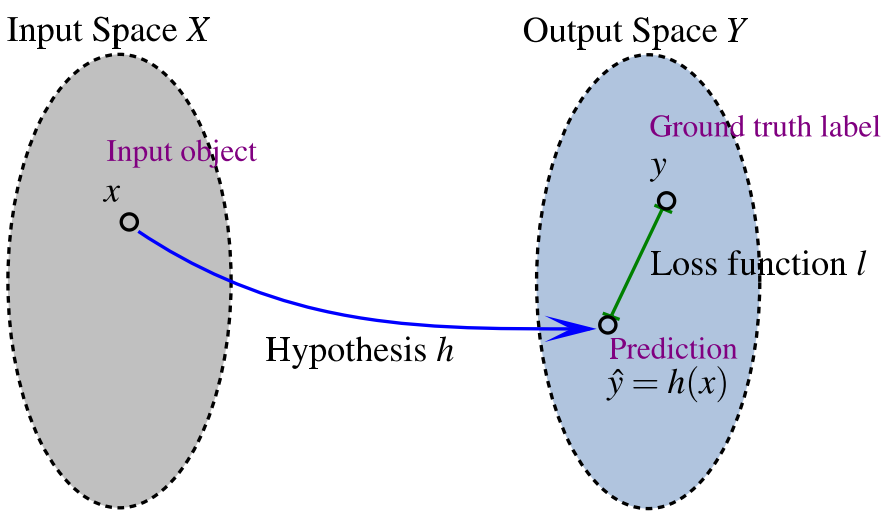
\includegraphics[scale=0.26]{gfx/descriminative_training}
\caption{Machine learning framework for Learning to Rank, obtained from Liu \cite{Liu2007}}
\label{fig:discriminative_training}
\end{figure}

Liu \cite{Liu2007} proposes a more narrow definition and only considers ranking methods to be a Learning to Rank method when it is \emph{feature based} and uses \emph{discriminative training}, in which the concepts \emph{feature based} and \emph{discriminative training} are itself defined as:
\begin{description}
\item[Feature Based]{means that all documents under investigation are represented by feature vectors. Those feature vectors reflect the relevance of the documents to the query, or the importance of the document in itself.}
\item[Discriminative Training]{means that the learning process can be well described by the four components of discriminative learning. That is, a Learning to Rank method has its own \emph{input space}, \emph{output space}, \emph{hypothesis space}, and \emph{loss function}, like the machine learning process described by Figure \ref{fig:discriminative_training}. \emph{Input space}, \emph{output space}, \emph{hypothesis space}, and \emph{loss function} are hereby defined as follows:
	\begin{description}
	\item[Input Space]{contains the objects under investigation. Usually objects are represented by feature vectors, extracted according to different applications.}
	\item[Output Space]{contains the learning target with respect to the input objects.}
	\item[Hypothesis Space]{defines the class of functions mapping the input space to the output space. The functions operate on the feature vectors of the input object, and make predictions according to the format of the output space.}
	\item[Loss Function]{in order to learn the optimal hypothesis, a training set is usually used, which contains a number of objects and their ground truth labels, sampled from the product of the input and output spaces. A loss function calculates the difference between the predictions $\hat{y}$ and the ground truth labels on a given set of data.
	\end{description}
	}
\end{description}


Figure \ref{fig:ltr_framework} shows how the machine learning process as described in Figure \ref{fig:discriminative_training} typically takes place in a ranking scenario. A set of queries $q_i$ with $n > i > 1$, the documents associated with these queries which are represented by feature vector $x_i$, and the relevant judgements of those documents $y_i$ are used together to train a model $h$. Model $h$ can after training be used to predict a ranking of the documents $y_i$, such the difference between the document rankings predicted by $h$ and the actual optimal rankings based on $y_i$ is minimal in terms of a loss function.
\begin{figure}[!h]
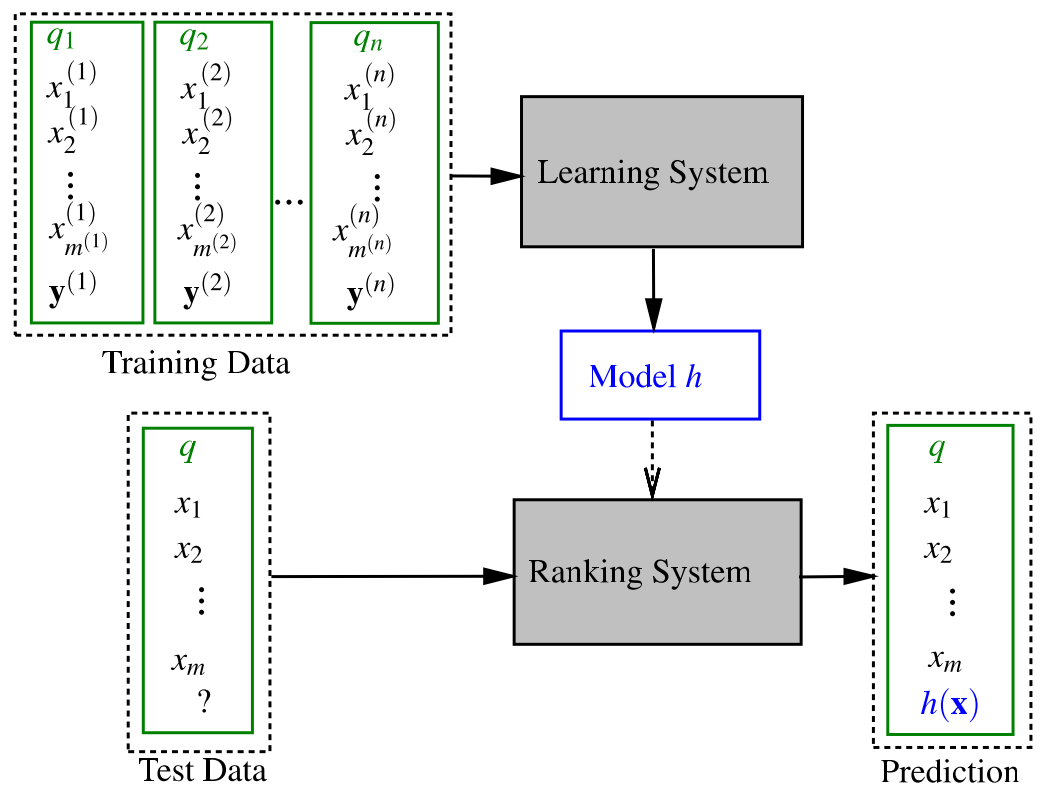
\includegraphics[scale=0.25]{gfx/ltr_framework}
\caption{A typical Learning to Rank setting, obtained from Liu \cite{Liu2007}}
\label{fig:ltr_framework}
\end{figure}\\

The predictions and the loss function might either be defined for:
\begin{enumerate}
\item the relevance of a single document
\item the classification of the most relevant document out of a document-pair
\item the ranking of documents directly
\end{enumerate}
\smallskip
These three approaches are in literature respectively labelled the pointwise approach, the pairwise approach and the listwise approach. These three approaches to Learning to Rank will be described in more detail in section \ref{sec:ltr_approaches}.

\section{How to evaluate a ranking}
\label{sec:how_to_evaluate_a_ranking}
Evaluation metrics have long been studied in the field of information retrieval. First in the form of evaluation of unranked retrieval sets and later, when the information retrieval field started focussing more on ranked retrieval, in the form of ranked retrieval evaluation. In this section several frequently used evaluation metrics for ranked results will be described.\\

No single evaluation metric that we are going to describe is indisputably better or worse than any of the other metrics. Different benchmarking settings have used different evaluation metrics. Metrics introduced in this section will be used in chapters \ref{chap:benchmark_results} and \ref{chap:cross_comparison} of this thesis to compare Learning to Rank methods in terms of ranking accuracy.
\subsection{Normalized Discounted Cumulative Gain}
Cumulative gain, or its successor discounted cumulative gain and normalized discounted cumulative gain, is one of the most widely used measures for effectiveness of ranking methods.
\subsubsection{Discounted Cumulative Gain}
There are two definitions of \ac{DCG} used in practice. \ac{DCG} at position $p$ was originally defined by J{\"a}rvelin and Kek{\"a}l{\"a}inen \cite{Jarvelin2002} as\\

$DCG_p = \sum\nolimits_{i=1}^p \frac{rel_i-1}{log_2(i+1)}$\\

with $rel_i$ the graded relevance of the result at position $i$. The idea is that highly relevant documents that appear lower in a search result should be penalized (discounted). This discounting is done by reducing the graded relevance  logarithmically proportional to the position of the result.\\

Burges et al. \cite{Burges2005} proposed an alternative definition of \ac{DCG} that puts stronger emphasis on document relevance\\

$DCG_p = \sum\nolimits_{i=1}^p \frac{2^{rel_i-1}}{log_2(i+1)}$\\

\subsubsection{Normalized Discounted Cumulative Gain}
\ac{NDCG} normalizes the \ac{DCG} metric to a value in the [0,1] interval by dividing by the \ac{DCG} value of the optimal rank. This optimal rank is obtained by sorting documents on relevance for a given query. The definition of \ac{NDCG} can be written down mathematically as\\

$nDCG_p = \frac{DCG_p}{IDCG_p}$\\

Table \ref{tab:example_calculation_NDCG} shows an example calculation for \ac{NDCG} for both the J{\"a}rvelin and Kek{\"a}l{\"a}inen \cite{Jarvelin2002} and Burges et al. \cite{Burges2005} version of \ac{DCG}.\\

\begin{table}[!h]
\begin{tabular}{llllllllllll}
 & \multicolumn{10}{c}{Rank} &  \\ 
\cline{2-11}
 & 1 & 2 & 3 & 4 & 5 & 6 & 7 & 8 & 9 & 10 & Sum \\ 
\hline
\hline
rel(i) & 10 & 7 & 6 & 8 & 9 & 5 & 1 & 3 & 2 & 4 &  \\
\hline
$\frac{2^{rel_i-1}}{log_2(i+1)}$ & 512 & 40.4 & 16 & 55.1 & 99.0 & 5.7 & 0.3 & 1.3 & 0.6 & 2.3 & 732.7 \\
\hline
$\frac{rel_i}{log_2(i+1)}$ & 10 & 4.42 & 3 & 3.45 & 3.48 & 1.78 & 0.33 & 0.95 & 0.6 & 1.16 & 29.17 \\  
\hline
\hline
optimal rank & 10 & 9 & 8 & 7 & 6 & 5 & 4 & 3 & 2 & 1 &  \\
\hline 
$\frac{2^{rel_i-1}}{log_2(i+1)}$ & 512 & 161.5 & 64 & 27.6 & 12.4 & 5.7 & 2.7 & 1.3 & 0.6 & 0.2 & 788.0 \\
\hline
$\frac{rel_i}{log_2(i+1)}$ & 10 & 5.68 & 4 & 3.01 & 2.32 & 1.78 & 1.33 & 0.95 & 0.6 & 0.29 & 29.96 \\   
\hline
 &  &  &  &  &  &  &  &  &  &  &  \\
 & \multicolumn{10}{c}{Burges \cite{Burges2005} et al. \ac{NDCG} = $\frac{732.7}{788.0} = 0.9298$} &  \\ 
  & \multicolumn{10}{c}{J{\"a}rvelin and Kek{\"a}l{\"a}inen \cite{Jarvelin2002} \ac{NDCG} = $\frac{29.17}{29.96} = 0.9736$} &  \\
\end{tabular}
\caption{Example calculation of \acs{NDCG}}
\label{tab:example_calculation_NDCG}
\end{table}

One limitation of \ac{NDCG} that it does not penalise for missing documents in the result set. \acl{NDCG} is often used with a fixed set size for the result set to mitigate the missing document problem. \ac{NDCG} with a fixed set size is often called \ac{NDCG}@k, where $k$ represents the set size.

\subsection{Expected Reciprocal Rank}
\ac{ERR} \cite{Chapelle2009} was designed based on the observation that \ac{NDCG} is based on the false assumption that the usefulness of a document at rank $i$ is independent of the usefulness of the documents at rank less than $i$. \ac{ERR} is based on the reasoning that users are likely to stop exploring the result list once they have found a document that satisfied their information need. The \ac{ERR} metric is defined as the expected reciprocal length of time that the user will take to find a relevant document. \ac{ERR} is formally defined as\\

$ERR = \sum\nolimits_{r=1}^n \frac{1}{r} \prod\nolimits_{i=1}^{r-1}(1-R_i)R_i$\\

where the product sequence part of the formula represents the chance that the user will stop at position $r$.\\
The algorithm to compute \ac{ERR} is shown in Listing \ref{alg:err}. The algorithm requires relevance grades $g_i$, $1 \le i \le n$ and mapping function $R$ that maps relevance grades to probability of relevance.

\LinesNumbered
\begin{algorithm}[H]
 $p \leftarrow 1, ERR \leftarrow 0$\\
 \For{$r\leftarrow 1$ \KwTo $n$}{
	$R \leftarrow R(g[r])$\\
	$ERR \leftarrow ERR + p * \frac{R}{r}$\\
	$p \leftarrow p * (1-R)$
 }
 Output $ERR$
 \caption{The algorithm for computation of the \acs{ERR} metric, obtained from \cite{Chapelle2009}}
 \label{alg:err}
\end{algorithm}

\subsection{Mean Average Precision}
\ac{AP} \cite{Zhu2004} is an often used binary relevance judgement based metric that can be seen as a trade-off between precision and recall that is defined as\\

$AP = \frac{\sum\nolimits_{k=1}^{n}Precision(k)*relevance(k)}{\text{number of relevant docs}}$\\

With $k$ being the positions in the result set between 1 and $n$. Table \ref{tab:example_calculation_AP} provides an example calculation of average precision where de documents at positions 1, 5, 6 and 8 in the ranking are relevant. The total number of available relevant documents in the document set \emph{R} is assumed to be seven.
\ac{MAP} is the average \ac{AP} for a set of queries.\\

$MAP = \frac{\sum\nolimits_{q=1}^{Q}AP(q)}{Q}$\\

\begin{table}
\begin{tabular}{lllllllllllll}
 & \multicolumn{10}{c}{Rank} &  & Sum \\ 
\cline{2-11}
 & 1 & 2 & 3 & 4 & 5 & 6 & 7 & 8 & 9 & 10 &  &  \\ 
\hline
$r_i$ & 1 & 0 & 0 & 0 & 1 & 1 & 0 & 1 & 0 & 0 &  &  \\ 
P@$i$ & 1 &  &  &  & 0.4 & 0.5 &  & 0.5 &  &  &  & 2.4 \\ 
\hline
 &  &  &  &  &  &  &  &  &  & \# of relevant docs & = & 7 \\ 
 &  &  &  &  &  &  &  &  &  & AP@10 & = & 0.34 \\ 
\end{tabular}
\caption{Average Precision example calculation.}
\label{tab:example_calculation_AP}
\end{table}

\section{Approaches to Learning to Rank}
\label{sec:ltr_approaches}
\subsection{Pointwise Approach}
The pointwise approach can be seen as the most straightforward way of using machine learning for ranking. Pointwise Learning to Rank methods directly apply machine learning methods to the ranking problem by observing each document in isolation. They can be subdivided in the following approaches:
	\begin{enumerate}
	\item regression-based, which estimate the relevance of a considered document using a regression model.
	\item classification-based, which classify the relevance category of the document using a classification model.
	\item ordinal regression-based, which classify the relevance category of the document using a classification model in such a way that the order of relevance categories is taken into account. 
	\end{enumerate}
Well-known algorithms that belong to the pointwise approach include McRank \cite{Li2007} and PRank \cite{Crammer2001}.
\subsection{Pairwise Approach}
Pointwise Learning to Rank methods have the drawback that they optimise real valued expected relevance, while evaluation metrics like \ac{NDCG} and \ac{ERR} are only impacted by a change in expected relevance when that change impacts a pairwise preference. The pairwise approach solves this drawback of the pointwise approach by regarding ranking as pairwise classification.\\

Aggregating a set of predicted pairwise preferences into the corresponding optimal rank is shown to be a NP-Hard problem \cite{Feldman2012}. An often used solution to this problem is to upper bound the number of classification mistakes by an easy to optimise function \cite{Bartlett2006}.\\

Well-known pairwise Learning to Rank algorithms include FRank \cite{Tsai2007}, GBRank \cite{Zheng2007}, LambdaRank \cite{Burges2006}, RankBoost \cite{Freund2003}, RankNet \cite{Burges2005}, Ranking \acs{SVM} \cite{Herbrich1999b,Joachims2002}, and SortNet \cite{Rigutini2008}.
\subsection{Listwise Approach}
Listwise ranking optimises the actual evaluation metric. The learner learns to predict an actual ranking itself without using an intermediate step like in pointwise or pairwise Learning to Rank. The main challenge in this approach is that most evaluation metrics are not differentiable. \ac{MAP}, \ac{ERR} and \ac{NDCG} are non-differentiable, non-convex and discontinuous functions, what makes them very hard to optimize.\\

Although the properties of \ac{MAP}, \ac{ERR} and \ac{NDCG} are not ideal for direct optimisation, some listwise approaches do focus on direct metric optimisation \cite{Yue2007, Taylor2008, Chapelle2010}. Most listwise approaches work around optimisation of the non-differentiable, non-convex and discontinuous metrics by optimising surrogate cost functions that mimic the behaviour of \ac{MAP}, \ac{ERR} or \ac{NDCG}, but have nicer properties for optimisation.\\

Well-known algorithms that belong to the listwise approach include AdaRank \cite{Xu2007}, BoltzRank \cite{Volkovs2009}, ListMLE \cite{Xia2008}, ListNet \cite{Cao2007}, RankCosine \cite{Qin2008}, SmoothRank \cite{Chapelle2010}, SoftRank \cite{Taylor2008}, \acs{SVM}$^{map}$ \cite{Yue2007}.

\section{Cross-validation experiments}
\label{sec:cross_validation}
A cross-validation experiment \cite{kohavi1995}, sometimes called rotation estimation, is an experimental set-up for model evaluation where the data is split into $k$ chunks of approximately equal size, called \emph{folds}. One of the folds is used as validation set, one of the folds is used as test set, and the rest of the $k - 2$ folds are used as training data. This procedure is repeated $k$ times, such that each fold is once used for validation, once as test set, and $k - 2$ times as training data. The performance can be measured in any model evaluation metric, and is averaged over the model performances on each of the folds. The goal of cross-validation is to define a data set to test the model in the training phase, in order to limit the problem of overfitting.\\

Cross-validation is one of the most frequently used model evaluations methods in the field of Machine Learning, including the Learning to Rank subfield. Often, folds in a cross-validation are created in a \emph{stratified} manner, meaning that the folds are created in such a way that the distributions of the target variable are approximately identical between the folds.

\section{An introduction to the MapReduce programming model}
MapReduce \cite{Dean2004} is a programming model invented at Google, where users specify a \emph{map} function that processes a key/value pair to generate a set of intermediate key/value pairs, and a \emph{reduce} function that merges all intermediate values associated with the same intermediate key. This model draws its inspiration from the field of functional programming, where \emph{map} and \emph{reduce} are commonly used functions.\\

This combination of the \emph{map} and \emph{reduce} functions allows for parallel computation. In the \emph{map} phase parallel computation can be performed by simply splitting the input data after a certain number of bytes, where each worker nodes performs the user-specified \emph{map}-function on its share of the data. Before the \emph{reduce} phase these intermediate answers of the different worker nodes are transformed in such a way that they are grouped by key value, this is called the shuffle-phase. After the shuffle-phase, the user-defined \emph{reduce}-function is applied to each group of key/value pairs in the reduce phase. Since the key/value pairs are already grouped by key in the shuffle phase, this \emph{reduce}-function can be applied to a group of key/value pairs on any of the worker nodes.\\
%\addtocontents{toc}{\protect\clearpage} % <--- just debug stuff, ignore
%\include{multiToC} % <--- just debug stuff, ignore for your documents
\chapter{Related Work}
\include*{Chapters/RelatedWork}

\chapter{Benchmark results}
\include*{Chapters/BenchmarkResults}
\chapter{Cross Benchmark Comparison}
\label{chap:cross_comparison}
As we have seen in Chapter~\ref{chap:benchmark_results}, the evaluation of Learning to Rank methods is spread over several benchmark data sets. However, as the Learning to Rank methods evaluated differs between benchmarks, no single benchmark comparison can be regarded as a conclusive argument on which Learning to Rank method is most accurate.\\

Several studies make a small start in considering Learning to Rank methods performance over multiple benchmark data sets. Gomes et al. \cite{Gomes2013} analysed ranking accuracy of a set of models on both LETOR 3.0 and LETOR 4.0. Busa-Fekete et al. \cite{Busa-Fekete2013} compared the accuracy of a small set of models over the LETOR 4.0 data sets, both MSLR data sets, both Yahoo! Learning to Rank Challenge data sets and the OHSUMED dataset from LETOR 3.0. To our knowledge, no structured meta-analysis on ranking accuracy has been conducted where evaluation results on several benchmark collections are taken into account. With a meta-analysis we will compare the performance of Learning to Rank methods across the Learning to Rank benchmark data sets described in foregoing sections.

\section{Collecting Evaluation Results}
\label{sec:collecting_evaluation_results}
With a literature review we will collect evaluation results on the data sets / collections. The following list presents an overview of the benchmark collections taken into account in the meta-analysis:
\begin{itemize}
\item LETOR 2.0
\item LETOR 3.0
\item LETOR 4.0
\item Yahoo! Learning to Rank Challenge
\item Yandex Internet Mathematics Competition 2009
\item MSLR-web10/30k
\item WCL2R
\item AOL
\end{itemize}

For the LETOR collections, the evaluation results of the baseline models will be used from LETOR 2.0\footnote{http://research.microsoft.com/en-us/um/beijing/projects/letor/letor2.0/baseline.aspx}, LETOR 3.0\footnote{http://research.microsoft.com/en-us/um/beijing/projects/letor/letor3baseline.aspx} and LETOR 4.0\footnote{http://research.microsoft.com/en-us/um/beijing/projects/letor/letor4baseline.aspx} as listed on the LETOR website.\\

LETOR 1.0, LETOR 3.0, Yahoo! Learning to Rank Challenge, WCL2R and AOL have accompanying papers which were published together with these benchmark collections. Users of those benchmark collections are encouraged to cite these papers. Therefore, we collect evaluation measurements of Learning to Rank methods on these benchmark collections through forward literature search. Table~\ref{tbl:ltr_benchmark_forref} presents an overview of the results of this forward literature search. Google Scholar will be used to perform the forward reference search.

\begin{table}[!h]
\begin{tabular}{l|l|l}
Benchmark & Paper & \# of forward references \\
\hline
LETOR 1.0 \& 2.0 & Liu et al. \cite{Liu2007b} & 307\\
LETOR 3.0 & Qin et al. \cite{Qin2010} & 105\\
Yahoo! Learning to Rank Challenge & Chapelle et al. \cite{Chapelle2011a} & 102\\
AOL dataset & Pass et al. \cite{Pass2006} & 339\\
WCL2R & Alc{\^a}ntara et al. \cite{Alcantara2010} & 2\\
\end{tabular}
\caption{Forward references of Learning to Rank benchmark papers}
\label{tbl:ltr_benchmark_forref}
\end{table}

The LETOR 4.0, MSLR-web10/30k and Yandex Internet Mathematics Competition 2009 benchmark collections were not accompanied with a describing study. To collect measurements of Learning to Rank methods evaluated on these benchmarks, a Google Scholar search is performed on the name of the benchmark. Table~\ref{chap:benchmark_results} shows the results of this literature search.

\begin{table}[!h]
\begin{tabular}{l|l}
Benchmark & Google Scholar search results \\
\hline
LETOR 4.0 & 75 results \\
MSLR-web10k & 16 results \\
MSLR-web30k & 15 results \\
Yandex Internet Mathematics Competition & 1 result \\ 
\end{tabular}
\caption{Google Scholar search results statistics for Learning to Rank benchmarks}
\label{tbl:ltr_benchmark_searchres}
\end{table}

\section{Comparison Methodology}
The LETOR 3.0 paper \cite{Qin2010} states that it may differ between data sets what the most accurate ranking methods are. To evaluate the overall performance of Learning to Rank methods over the multiple data sets in the LETOR 3.0 collections, Qin et al. \cite{Qin2010} proposed a measure called \emph{winning number} as the number of other algorithms that an algorithm can beat over the set of data sets. Formally the winning number measure is defined as\\

$\text{Winning Number}_i(M) = \sum\nolimits_{j=1}^n \sum\nolimits_{k=1}^m I_{\{M_i(j)>M_k(j)\}}$\\

where $j$ is the index of a dataset, $n$ the number of data sets in the comparison, $i$ and $k$ are indices of an algorithm, $M_i(j)$ is the performance of the $i$-th algorithm on the $j$-th dataset, $M$ is a ranking measure (such as \ac{NDCG} or \ac{MAP}), and $I_{\{M_i(j)>M_k(j)\}}$ is an indicator function such that\\

$I_{\{M_i(j)>M_k(j)\}} = \begin{cases}
1 & \text{if } M_i(j) > M_k(j), \\
0 & \text{otherwise}
\end{cases}$\\

In contrast to the winning number comparison on LETOR 3.0, there will not be accuracy measurements for each algorithm on each dataset in our meta-analysis. To compare algorithms based on a sparse set of evaluation measurements, a normalised version of the Winning Number metric will be used. This \ac{NWN} takes only those data sets into account that an algorithm is evaluated on and divides this by the theoretically highest Winning Number that an algorithm would have had in case it it would have been the most accurate algorithm on all data sets on which it has been evaluated. We will redefine the indicator function $I$ in order to only take into account those data sets that an algorithm is evaluated on, as \\

$I_{\{M_i(j)>M_k(j)\}} = \begin{cases}
1 & \text{if } M_i(j) \text{ and } M_k(j) \text{ are both defined and } M_i(j) > M_k(j), \\
0 & \text{otherwise}
\end{cases}$\\

From now on this adjusted version of Winning Number will be referred to as \ac{NWN}. The mathematical definition of \ac{NWN} is\\

$\text{Normalised Winning Number}_i(M) = \frac{\text{Winning Number}_i(M)}{\text{Ideal Winning Number}_i(M)}$\\

\noindent
where \ac{IWN} is defined as\\

$\text{Ideal Winning Number}_i(M) = \sum\nolimits_{j=1}^n \sum\nolimits_{k=1}^m D_{\{M_i(j),M_k(j)\}}$\\

where $j$ is the index of a dataset, $n$ the number of data sets in the comparison, $i$ and $k$ are indices of an algorithm, $M_i(j)$ is the performance of the $i$-th algorithm on the $j$-th dataset, $M$ is a ranking measure (such as \ac{NDCG} or \ac{MAP}), and $D_{\{M_i(j),M_k(j)\}}$ is an evaluation definition function such that\\

$D_{\{M_i(j),M_k(j)\}} = \begin{cases}
1 & \text{if } M_i(j) \text{ and } M_k(j) \text{ are both defined}, \\
0 & \text{otherwise}
\end{cases}$\\

\ac{NDCG}@3, \ac{NDCG}@5, \ac{NDCG}@10 and \ac{MAP} are chosen as metrics on which the meta-analysis will be performed. These metrics seem to be the most frequently used evaluation metrics in most of the used benchmark data sets. An exception is the Yahoo! Learning to Rank Challenge data sets on which mainly \ac{ERR} is used as main evaluation metric. The lack of use of the \ac{ERR}-metric in other benchmarks makes it unsuitable for a cross-benchmark comparison. By making the decision to include \ac{NDCG} at three cut-off points and only a single \ac{MAP} entry, we implicitly attain a higher weight for \ac{NDCG} compared to \ac{MAP} on an analysis that combines all measurements on the four metrics. This implicit weighting is arbitrary and therefore undesirable, but the number of algorithm evaluation results gained by this makes it a pragmatic approach.

\section{Evaluation Results Found in Literature}
Table \ref{tab:ltr_methods_used} gives an overview of the Learning to Rank methods for which evaluation results were found for one or more of the benchmark data sets listed in section~\ref{sec:collecting_evaluation_results} through the literature review process also described in section~\ref{sec:collecting_evaluation_results}. Occurrences of L2, L3 and L4 in Table \ref{tab:ltr_methods_used} imply that these algorithms are evaluated as official LETOR 2.0, LETOR 3.0 and LETOR 4.0 baselines respectively.\\

Some studies with evaluation results found through in literature review were not usable for the meta-analysis. The following enumeration lists those properties that made one or more studies unusable for the meta-analysis. Between brackets are the studies that these properties apply to.

\begin{enumerate}
\item A different evaluation methodology was used in the study compared to what was used in other studies using the same benchmark \cite{Geng2011, Lin2012}.
\item The study focussed on a different Learning to Rank task (e.g. rank aggregation or transfer ranking) \cite{De2011, De2010, Derhami2013, De2012, Chen2010, Ah-Pine2008, Wang2009c, De2013, Miao2013, Hoi2008, De2012b, Duh2011b, Argentini2012, Qin2010c, Volkovs2013, Desarkar2011, Pan2013, Lin2011b, Volkovs2012, Dammak2011}.
\item The study used an altered version of a benchmark that contained additional features \cite{Bidoki2009, Ding2010}.
\item The study provides no exact data of the evaluation results (e.g. results are only in graphical form) \cite{Wang2008, Wang2010, Xu2010, Kuo2009, Li2008, Xia2008, Zhou2011, Wu2011, Zhu2009, Karimzadehgan2011, Swersky2012, Pan2011, Ni2008, Ciaramita2008, Stewart2012, Petterson2009, Agarwal2010, Chang2009, Qin2008c, Adams2011, Sculley2009, Huang2008, Alejo2010, Sun2011, He2010b, Benbouzid2012, Geng2012, Chen2012, Xu2012, Shivaswamy2011}.
\item The study reported evaluation results in a different metric than the metrics chosen for this meta-analysis \cite{Yu2009, Thuy2009, Pahikkala2009, Kersting2009, Mohan2011}.
\item The study reported a higher performance on baseline methods than official benchmark runs \cite{Dubey2009, Banerjee2009, Peng2010b, Song2014, Bian2010, Bian2010b, Carvalho2008, Acharyya2012, Peng2010b, Tran2012, Asadi2013c}. Such cases are not necessarily caused by malicious intent, but might be caused by a mix-up of the two existing versions of the \ac{NDCG} metric (J{\"a}rvelin and Kek{\"a}l{\"a}inen \cite{Jarvelin2002} and Burges et al. \cite{Burges2005}). 
\item The study did not report any baseline performance that allowed us to check validity of the results \cite{Chakrabarti2008, Wang2012b, Buffoni2011}.
\end{enumerate}

\begin{table}[!h!p]
\scalebox{0.75}{
\begin{tabular}{|l|l|l||l|l|l|}
Method & Described & Evaluated & Method & Described & Evaluated \\
\hline 
AdaRank-\acs{MAP} & \cite{Xu2007} & L2, L3, L4 & Linear Regression & \cite{Cossock2006} & L3, \cite{Wang2012, Volkovs2011} \\ 
AdaRank-\acs{NDCG} & \cite{Xu2007} & L2, L3, L4,  \cite{Busa-Fekete2013,Tan2013} & List\acs{MLE} & \cite{Xia2008} & \cite{Lin2010, Lin2011, Gao2014} \\ 
ADMM & \cite{Duh2011} & \cite{Duh2011} & ListNet & \cite{Cao2007} & L2, L3, L4 \\ 
Approx\acs{AP} & \cite{Qin2010b} & \cite{Qin2010b} & ListReg & \cite{Wu2011} & \cite{Wu2011} \\ 
Approx\acs{NDCG} & \cite{Qin2010b} & \cite{Qin2010b} & LRUF & \cite{Torkestani2012b} & \cite{Torkestani2012b} \\ 
BagBoo & \cite{Pavlov2010} & \cite{Ganjisaffar2011c} & MCP & \cite{Laporte2013} & \cite{Laporte2013} \\ 
Best Single Feature &  & \cite{Gomes2013} & \acs{MHR} & \cite{Qin2007} & L2 \\ 
BL-MART & \cite{Ganjisaffar2011c} & \cite{Ganjisaffar2011c} & MultiStageBoost & \cite{Kao2013} & \cite{Kao2013} \\ 
BoltzRank-Single & \cite{Volkovs2009} & \cite{Volkovs2009, Volkovs2013} & NewLoss & \cite{Peng2010} & \cite{Peng2010} \\ 
BoltzRank-Pair & \cite{Volkovs2009} & \cite{Volkovs2009, Ganjisaffar2011c, Volkovs2013} & OWPC & \cite{Usunier2009} & \cite{Usunier2009} \\ 
BT & \cite{Zhou2008} & \cite{Zhou2008} & PERF-\acs{MAP} & \cite{Pan2011} & \cite{Torkestani2012b} \\ 
C-\acs{CRF} & \cite{Qin2008b} & \cite{Qin2008b} & PermuRank & \cite{Xu2008} & \cite{Xu2008} \\ 
CA & \cite{Metzler2007} & \cite{Busa-Fekete2013,Tan2013} & Q.D.\acs{KNN} & \cite{Geng2008} & \cite{Wang2013} \\ 
CCRank & \cite{Wang2011c} & \cite{Wang2011c} & RandomForest &  & \cite{Gomes2013} \\ 
CoList & \cite{Gao2014} & \cite{Gao2014} & Rank-PMBGP & \cite{Sato2013} & \cite{Sato2013} \\ 
Consistent-RankCosine & \cite{Ravikumar2011} & \cite{Tan2013} & RankAgg\acs{NDCG} & \cite{Wang2013} & \cite{Wang2013} \\ 
DCMP & \cite{Renjifo2012}  & \cite{Renjifo2012}  & RankBoost & \cite{Freund2003} & L2, L3, L4, \cite{Busa-Fekete2013, Alcantara2010} \\ 
DirectRank & \cite{Tan2013} & \cite{Tan2013} & RankCSA & \cite{He2010} & \cite{He2010} \\ 
Energy\acs{NDCG} & \cite{Freno2011} & \cite{Freno2011} & RankDE & \cite{Bollegala2011} & \cite{Sato2013} \\ 
FBPCRank & \cite{Lai2011} & \cite{Lai2011} & RankELM (pairwise) & \cite{Zong2013} & \cite{Zong2013} \\ 
FenchelRank & \cite{Lai2013} & \cite{Lai2013, Lai2013b, Laporte2013} & RankELM (pointwise) & \cite{Zong2013} & \cite{Zong2013} \\ 
FocusedBoost & \cite{Niu2012} & \cite{Niu2012} & RankMGP & \cite{Lin2012} & \cite{Lin2012} \\ 
FocusedNet & \cite{Niu2012} & \cite{Niu2012} & RankNet & \cite{Burges2005} & \cite{Busa-Fekete2013, Papini2012, Niu2012} \\ 
Focused\acs{SVM} & \cite{Niu2012} & \cite{Niu2012} & Rank\acs{RLS} & \cite{Pahikkala2009} & \cite{Pahikkala2010} \\ 
FP-Rank & \cite{Song2013} & \cite{Song2013} & Rank\acs{SVM} & \cite{Herbrich1999, Joachims2002} & L2, L3, \cite{Busa-Fekete2013, Freno2011, He2010, Alcantara2010} \\ 
FRank & \cite{Tsai2007} & L2, L3, \cite{Wang2012} & Rank\acs{SVM}-Primal &  & L3, \cite{Lai2011} \\ 
FSMRank & \cite{Lai2013c} & \cite{Lai2013c,Laporte2013} & Rank\acs{SVM}-Struct &  & L3, L4 \\
FSM$^{\acs{SVM}}$ & \cite{Lai2013c} & \cite{Lai2013c} & RCP & \cite{Elsas2008} & \cite{Elsas2008} \\ 
GAS-E & \cite{Geng2007} & \cite{Lai2013c} & RE-QR & \cite{Veloso2010} & \cite{Veloso2010} \\
\acs{GP} & \cite{DeAlmeida2007} & \cite{Alcantara2010} & REG-SHF-SDCG & \cite{Wu2009} & \cite{Wu2009} \\  
\acs{GP}Rank & \cite{Silva2009} & \cite{Torkestani2012} & Ridge Regression & \cite{Cossock2006} & L3 \\
GRank\acs{RLS} & \cite{Pahikkala2010} & \cite{Pahikkala2010} & RSRank & \cite{Sun2009} & \cite{Lai2013} \\ 
Group\acs{CE} & \cite{Lin2011} & \cite{Lin2011} & SmoothGrad & \cite{Le2007} & \cite{Tan2013} \\ 
Group\acs{MLE} & \cite{Lin2010} & \cite{Lin2011} & SmoothRank & \cite{Chapelle2010} & L3, \cite{Chapelle2010} \\
IntervalRank & \cite{Moon2010} & \cite{Moon2010, Freno2011} & SoftRank & \cite{Taylor2008, Guiver2008} & \cite{Qin2010b} \\ 
\acs{IP}Rank & \cite{Wang2009b} & \cite{Wang2009b, Torkestani2012} & SortNet & \cite{Rigutini2008} & \cite{Rigutini2008,Freno2011} \\
KeepRank & \cite{Chen2009} & \cite{Chen2009} & SparseRank & \cite{Lai2013b} & \cite{Lai2013b} \\ 
Kernel-\acs{PCA} RankBoost & \cite{Duh2008} & \cite{Duh2008, Sato2013} & \acs{SVD}-RankBoost & \cite{Lin2009} & \cite{Lin2009} \\
KL-\acs{CRF} & \cite{Volkovs2011} & \cite{Volkovs2011} & \acs{SVM}$^{\acs{MAP}}$ & \cite{Yue2007} & L3, \cite{Wang2012, Xu2008, Niu2012} \\ 
LAC-MR-OR & \cite{Veloso2008} & \cite{Veloso2008} & SwarmRank & \cite{Diaz-Aviles2009} & \cite{Sato2013} \\ 
LambdaMART & \cite{Burges2010} & \cite{Asadi2013a, Ganjisaffar2011c} & TGRank & \cite{Lai2013} & \cite{Lai2013} \\ 
LambdaNeuralRank & \cite{Papini2012} & \cite{Papini2012} & TM & \cite{Zhou2008} & \cite{Zhou2008, Papini2012, Tan2013} \\ 
LambdaRank & \cite{Burges2006} &  & VFLR & \cite{Cai2012} & \cite{Cai2012} \\ 
LARF & \cite{Torkestani2012} & \cite{Torkestani2012} &  &  &  \\ 
\end{tabular}}
\caption{An overview of Learning to Rank algorithms and their occurrence in evaluation experiments on benchmark data sets}
\label{tab:ltr_methods_used}
\end{table}

\section{Results \& Discussion}
The following subsections provide the performance of Learning to Rank methods in terms of \ac{NWN} for \ac{NDCG}@3, \ac{NDCG}@5, \ac{NDCG}@10 and \ac{MAP}. Performance of the Learning to Rank methods is plotted with \ac{NWN} on the vertical axis and the number of data sets on which the method has been evaluated on the horizontal axis. The further to the right, the more certain we can be about the performance of the Learning to Rank method. The methods for which it holds that there is no other method that has 1) a higher \ac{NWN} and 2) a higher number data sets evaluated, are identified as the best performing methods and are labelled with the name of the method.

\subsection{NDCG@3}
Figure \ref{fig:normalised_winning_number_NDCG3} shows the performance of Learning to Rank methods for the \ac{NDCG}@3 metric. Table \ref{tab:raw_data_norm_winnum_ndcg35} in Appendix \ref{app:norm_winnum_ndcg35} provides the raw \ac{NWN} data for the Learning to Rank methods for which \ac{NDCG}@3 evaluation results were available.\\

\begin{figure}[!h]
\centering
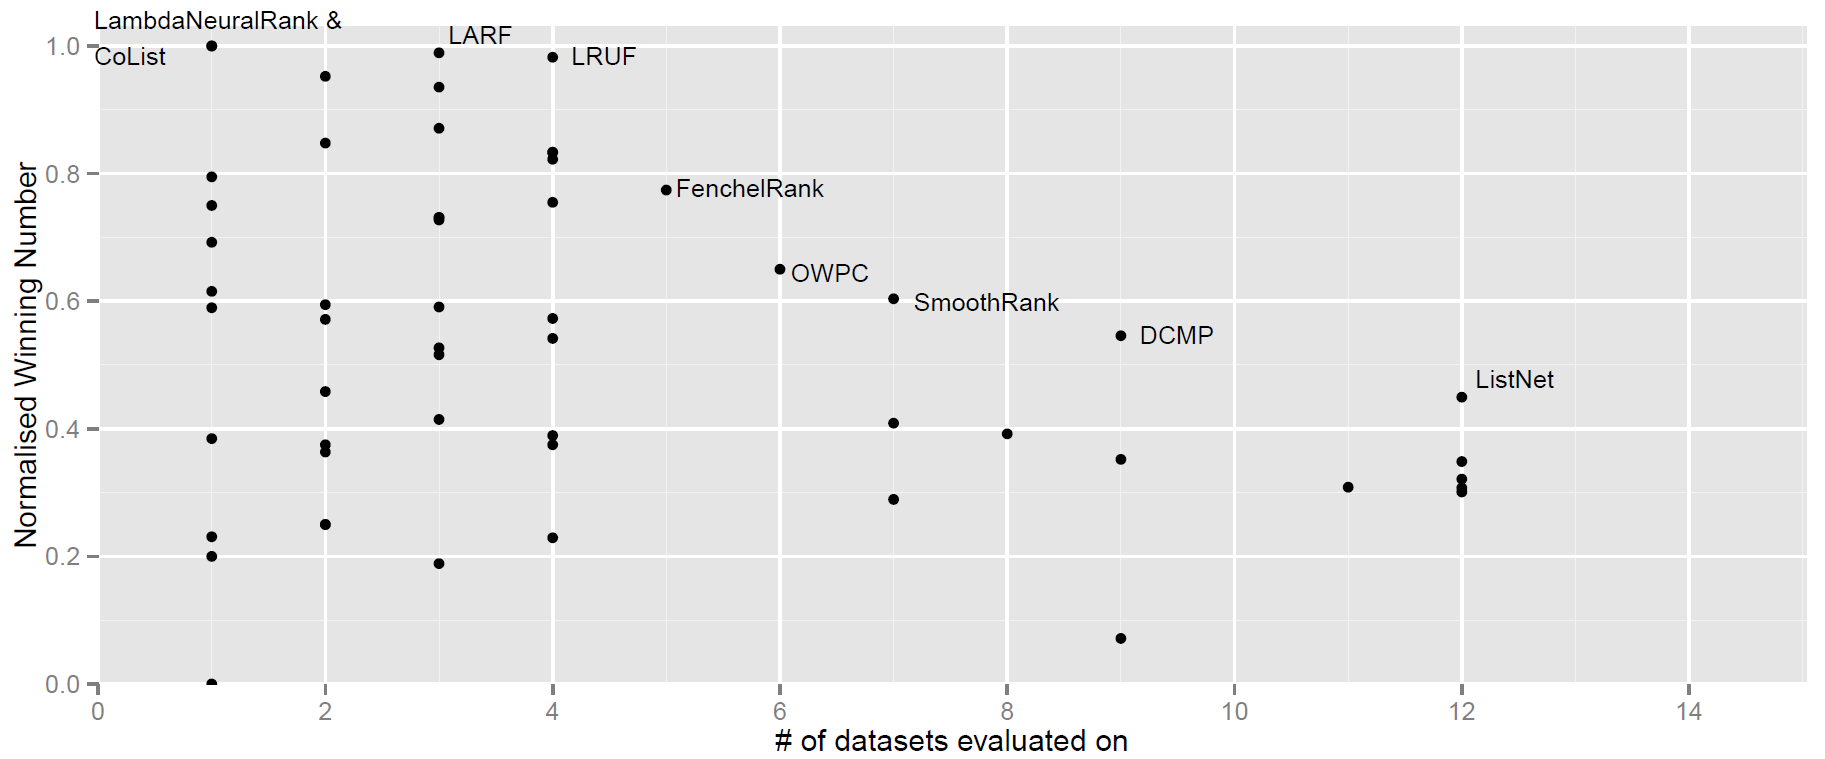
\includegraphics[scale=0.35]{gfx/ndcg3_winnum}
\caption{\acs{NDCG}@3 comparison of Learning to Rank methods}
\label{fig:normalised_winning_number_NDCG3}
\end{figure}

LambdaNeuralRank and CoList both acquired a perfect \ac{NWN} score of 1.0 by beating all other algorithms on one dataset, with LambdaNeuralRank winning on the AOL dataset and CoList winning on Yahoo! Set 2. LARF and LRUF both scored very high scores of near 1.0 on three of the LETOR 3.0 data sets, which can be said to have a higher degree of certainty on the methods' performance because they are validated on three data sets which in addition are more relevant data sets than AOL and Yahoo! Set 2 because there are more evaluation results available for the LETOR 3.0 data sets (see Table \ref{tab:ltr_methods_used}). FenchelRank, OWPC, SmoothRank, DCMP and ListNet are in that order increasingly lower in \ac{NWN}, but increasingly higher in number of data sets that they are evaluated on, resulting in a higher degree of certainty on the accuracy of the algorithms.\\

LambdaNeuralRank, CoList, LARF, LRUF, OWPC and DCMP evaluation results are all based on one study, therefore are subjected to the risk of one overly optimistic study producing those results. FenchelRank evaluation result are based combined result from two studies, although those studies have overlap in authors. SmoothRank and ListNet have the most reliable evaluation result source, as they were official LETOR baseline runs.  

\subsection{NDCG@5}
Figure \ref{fig:normalised_winning_number_NDCG5} shows the performance of Learning to Rank methods for the \ac{NDCG}@5 metric. Table \ref{tab:raw_data_norm_winnum_ndcg35} in Appendix \ref{app:norm_winnum_ndcg35} provides the raw Normalised Winning Number data for the Learning to Rank methods.\\

\begin{figure}[!h]
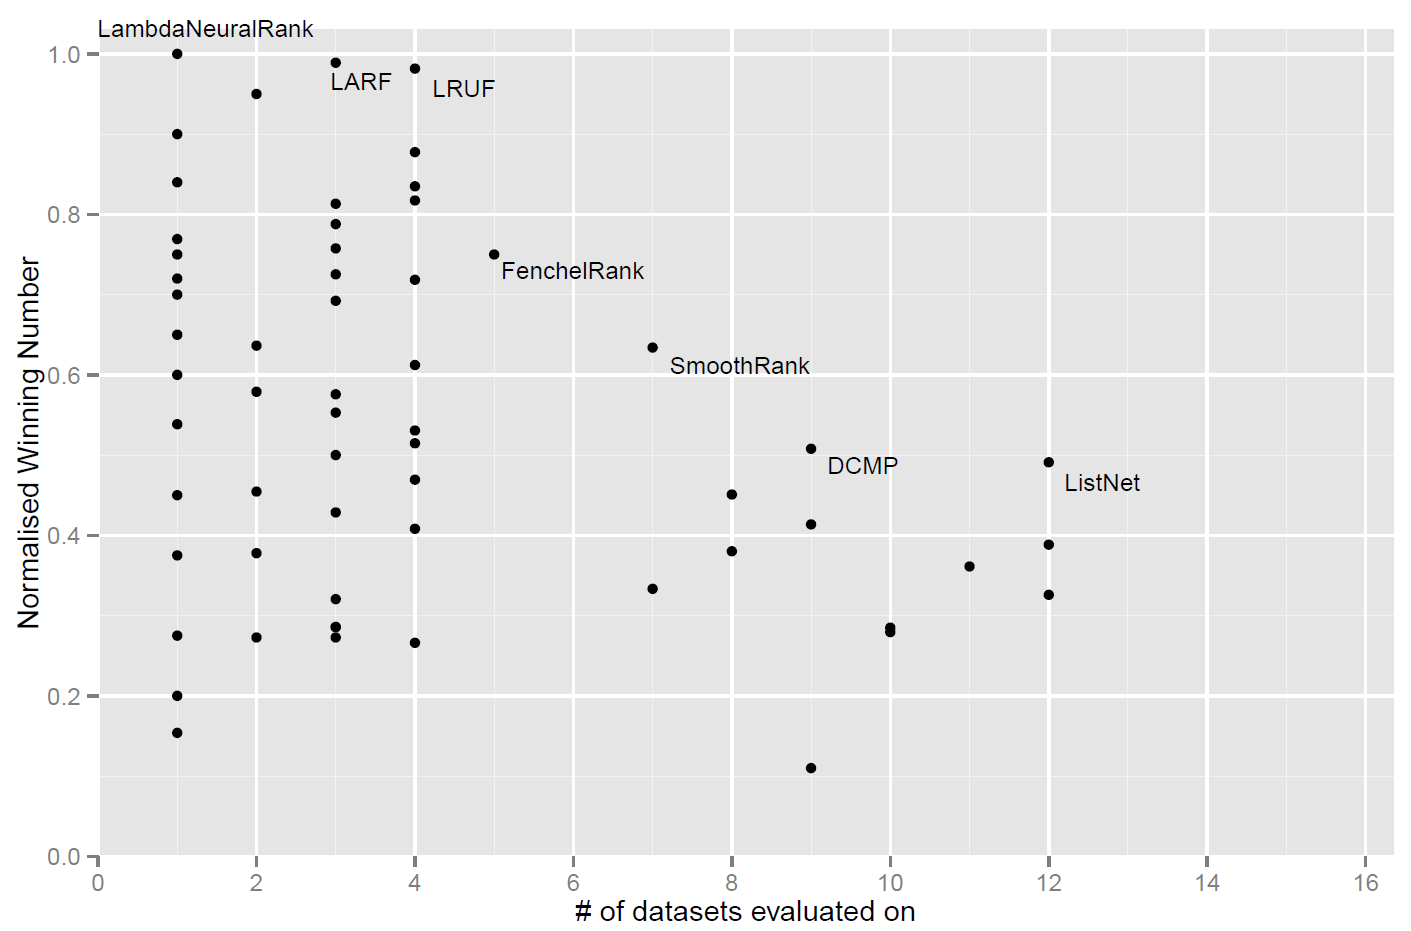
\includegraphics[scale=0.35]{gfx/ndcg5_winnum}
\caption{\acs{NDCG}@5 comparison of Learning to Rank methods}
\label{fig:normalised_winning_number_NDCG5}
\end{figure}

LambdaNeuralRank again beat all other methods solely with results on the AOL dataset scoring a \ac{NWN} of 1.0. LARF, LRUF, FenchelRank, SmoothRank, DCMP and ListNet are from left to right evaluated on an increasing number of data sets, but score decreasingly well in terms of \ac{NWN}. These results are highly in agreement with the \ac{NDCG}@3 comparison. The only modification compared to the \ac{NDCG}@3 comparison being that OWPC did show to be a method for which there were no methods performing better on both axes in the \ac{NDCG}@5 comparison, but not in the \ac{NDCG}@3 comparison. Like in the \ac{NDCG}@3 comparison, SmoothRank and ListNet can be regarded as most reliable results because the evaluation measurements for these methods are based on LETOR official baselines.

\subsection{NDCG@10}
Figure \ref{fig:normalised_winning_number_NDCG10} shows the performance of Learning to Rank methods for the \ac{NDCG}@10 metric. Table \ref{tab:raw_data_norm_winnum_ndcg10map} in Appendix \ref{app:norm_winnum_ndcg10map} provides the raw Normalised Winning Number data for the Learning to Rank methods.\\

\begin{figure}[!h]
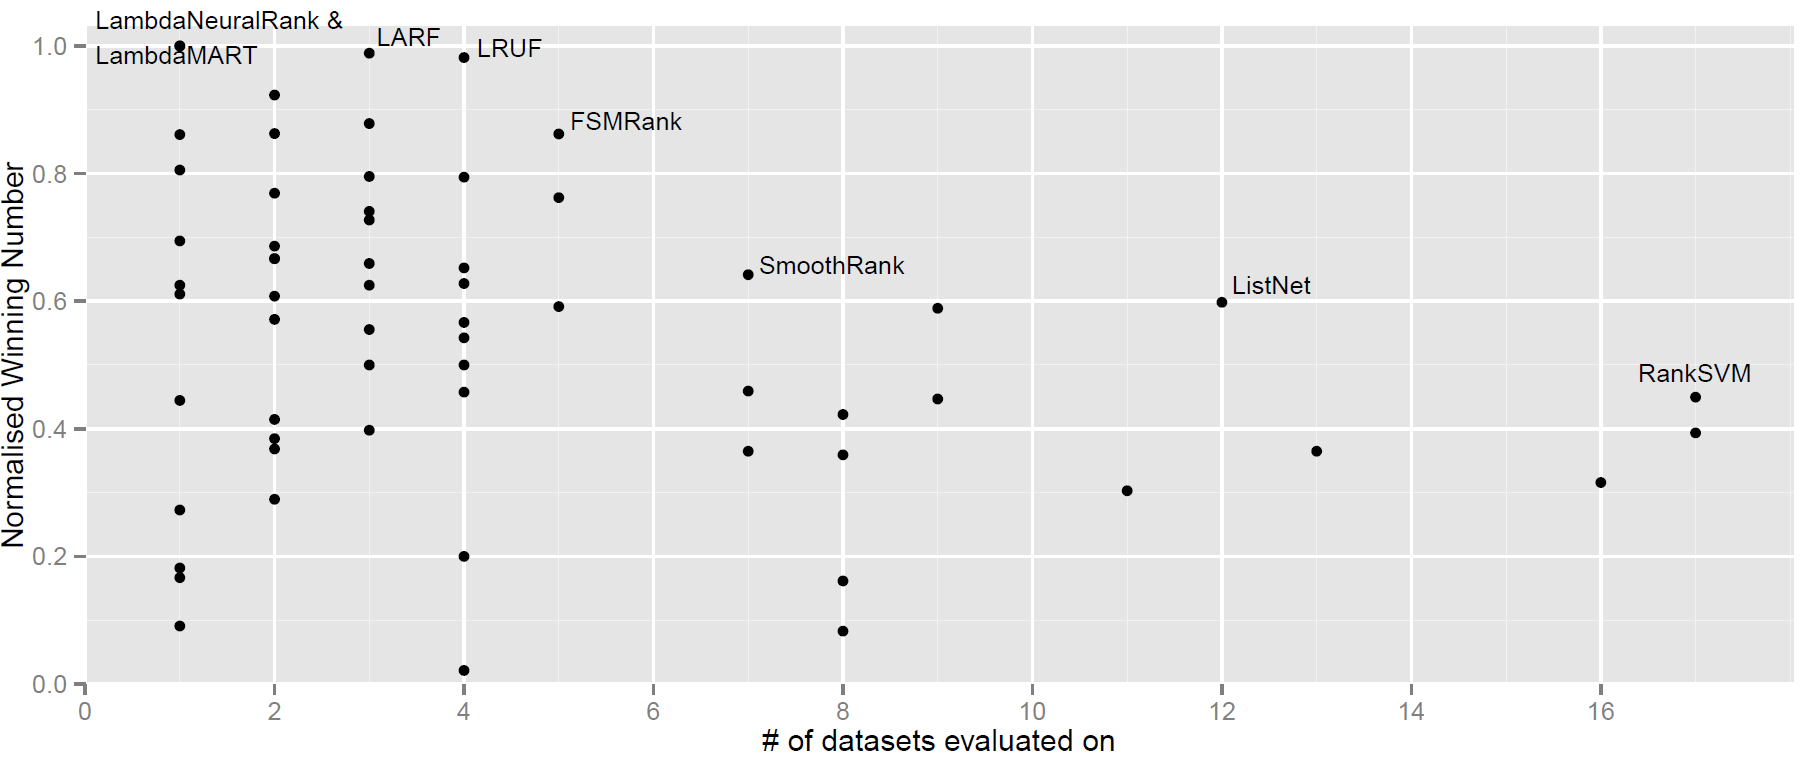
\includegraphics[scale=0.35]{gfx/ndcg10_winnum}
\caption{\acs{NDCG}@10 comparison of Learning to Rank methods}
\label{fig:normalised_winning_number_NDCG10}
\end{figure}

LambdaMART and LambdaNeuralRank score a \ac{NWN} of 1.0 on the \ac{NDCG}@10 comparison. For LambdaNeuralRank these results are again based on AOL dataset measurements. LambdaMART showed the highest \ac{NDCG}@10 performance for the MSLR-WEB10k dataset. The set of algorithms for which there is no other algorithm with both a higher \ac{NWN} and number of data sets evaluated on is partly in agreement with those for the \ac{NDCG}@3 and \ac{NDCG}@5 comparisons: {LARF, LRUF, FSMRank, SmoothRank, ListNet, RankSVM}. SmoothRank and FSMRank were not present in this set for the \ac{NDCG}@3 and \ac{NDCG}@5 comparison, but were close by, as can be seen in Tables \ref{tab:raw_data_norm_winnum_ndcg35} in Appendix \ref{app:norm_winnum_ndcg35}. DCMP is not in the set in contrast with the \ac{NDCG}@3 and \ac{NDCG}@5 comparison.

\subsection{MAP}
Figure \ref{fig:normalised_winning_number_map} shows the performance of Learning to Rank methods for the \ac{MAP} metric. Table \ref{tab:raw_data_norm_winnum_ndcg10map} in Appendix \ref{app:norm_winnum_ndcg10map} provides the raw \ac{NWN} data for the Learning to Rank methods.\\

\begin{figure}[!h]
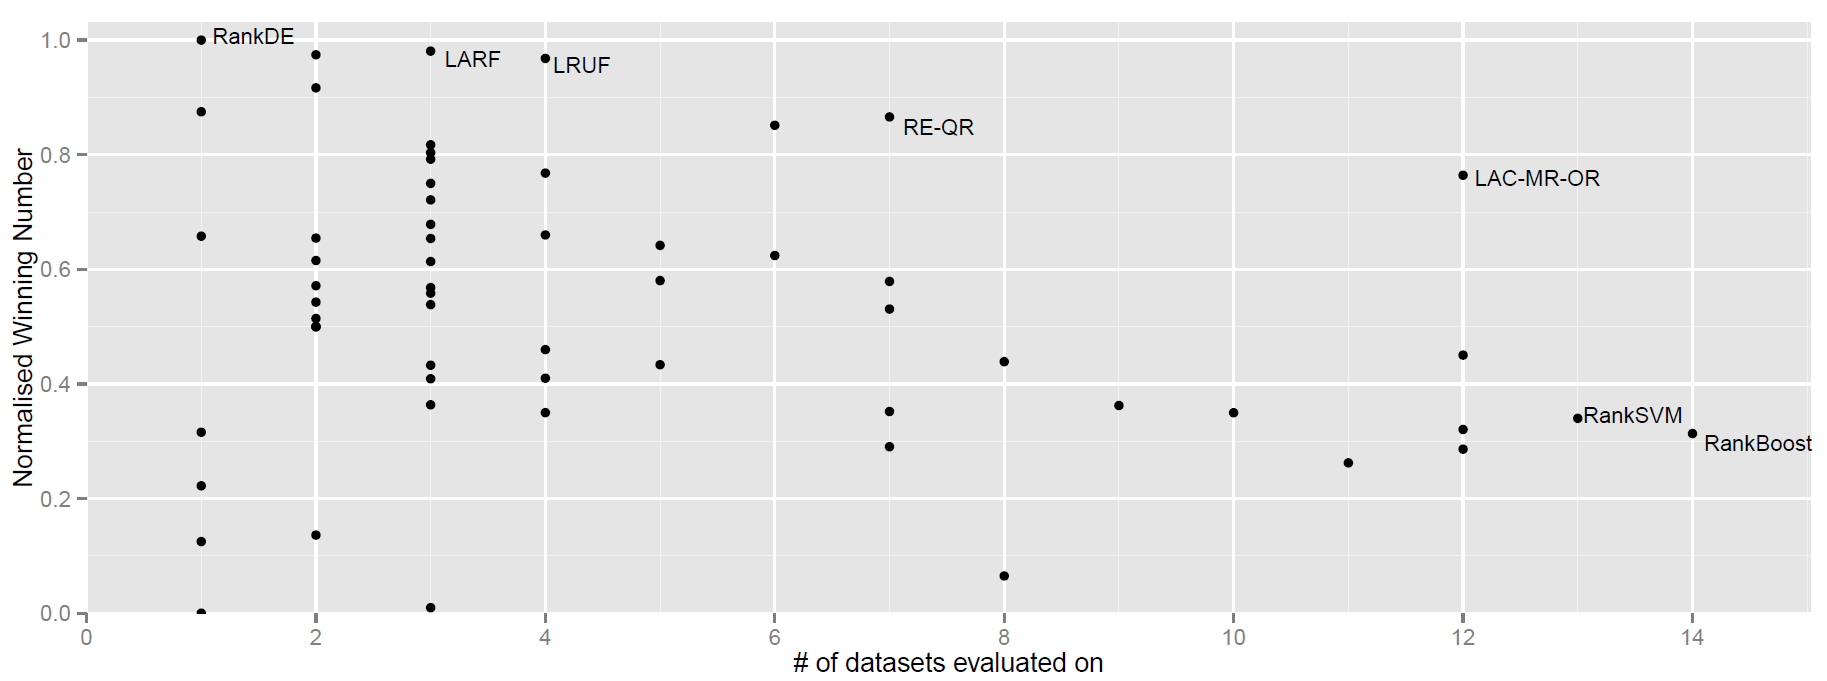
\includegraphics[scale=0.35]{gfx/map_winnum}
\caption{\acs{MAP} comparison of Learning to Rank methods}
\label{fig:normalised_winning_number_map}
\end{figure}

Where comparisons on the \ac{NDCG}-metric at different cut-off points where highly in agreement in terms of the best performing algorithms, the comparison in terms of \ac{MAP} shows different results. RankDE scores a \ac{NWN} of 1.0 on one dataset, like LambdaNeuralRank did on for all \ac{NDCG}-comparisons. In contrast to LambdaNeuralRank, RankDE achieved this highest score on the LETOR 2.0 TD2003, a dataset on which many methods are evaluated.\\

LARF and LRUF score very high \ac{NWN} scores, but based on only relatively few data sets, just as in the \ac{NDCG}-comparisons. Notable is that SmoothRank and ListNet, which showed both high accuracy and high certainty on all \ac{NDCG}-comparisons, are not within the best performing methods in the \ac{MAP}-comparison. A deeper look in the raw data Tables \ref{tab:raw_data_norm_winnum_ndcg35} and \ref{tab:raw_data_norm_winnum_ndcg10map} in Appendices \ref{app:norm_winnum_ndcg35} and \ref{app:norm_winnum_ndcg10map} respectively shows that LAC-MR-OR is evaluated on many more data sets for \ac{MAP} compared to \ac{NDCG}, which resulted in LAC-MR-OR obtaining equal certainty to ListNet with a higher \ac{NWN}. SmoothRank performed a \ac{NWN} of around 0.53 over 7 data sets, which is still good in both certainty and accuracy, but not among the top methods. RE-QR is one of the best performers in the \ac{MAP}-comparison with a reasonable amount of benchmark evaluations. No reported \ac{NDCG} performance was found in the literature study for RE-QR. There is a lot of certainty on the accuracy of RankBoost and Rank\acs{SVM} as both models are evaluated on the majority of data sets included in the comparison for the \ac{MAP}-metric, but given their \ac{NWN} it can said that both methods are not within the top performing Learning to Rank methods.

\subsection{Cross-metric}
Figure \ref{fig:normalised_winning_number_all} shows the \ac{NWN} as function of \ac{IWN} for the methods described in Table \ref{tab:ltr_methods_used}. Table \ref{tab:raw_data_norm_winnum_all} in Appendix \ref{app:norm_winnum_all} provide the raw data plotted in Figure \ref{fig:normalised_winning_number_all}.\\

\begin{figure}[!h]
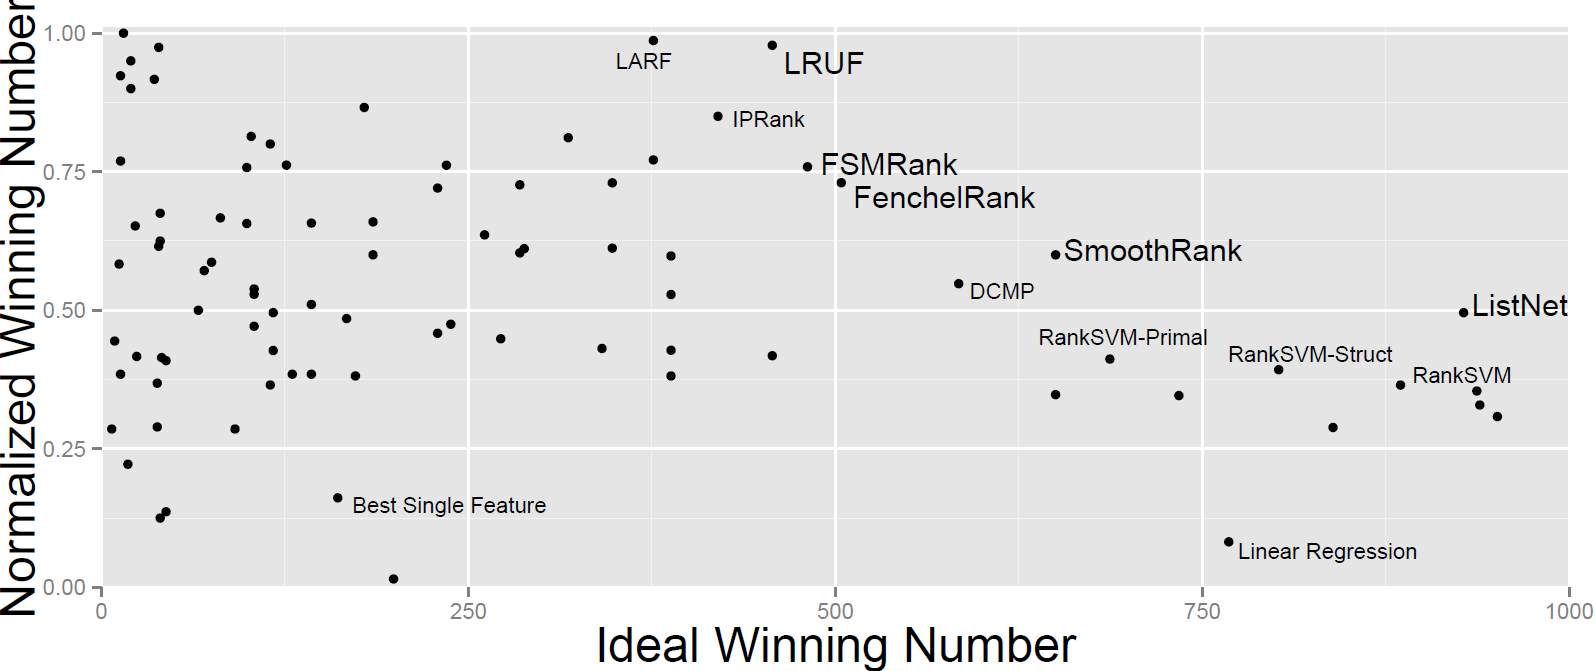
\includegraphics[scale=0.405]{gfx/combined_normalized_winnum}
\caption{Cross-benchmark comparison of Learning to Rank methods}
\label{fig:normalised_winning_number_all}
\end{figure}

The cross-metric comparison is based on the \ac{NDCG}@3, \ac{NDCG}@5, \ac{NDCG}@10 and \ac{MAP} comparisons combined, which justifies analysing the comparison more thoroughly. Figure \ref{fig:normalised_winning_number_all} labels the algorithms with no other algorithm having a higher value on both the horizontal axis and vertical axis, but also labels the algorithms with exactly one algorithm having a higher value on both axes with smaller font size. In addition, Linear Regression and the ranking method of simply sorting on the best single feature are labelled as baselines.\\

LRUF, FSMRank, FenchelRank, SmoothRank and ListNet showed to be the methods that have no other method superior to them in both \ac{IWN} and \ac{NWN}. LRUF is the only method that achieved this in all \ac{NDCG} comparisons, the \ac{MAP} comparison as well as the cross-metric comparison. With FenchelRank, FSMRank, SmoothRank and ListNet being among the top performing methods in all \ac{NDCG} comparisons as well as in the cross-metric comparison, it can be concluded that the cross-metric results are highly defined by the \ac{NDCG} performance as opposed to the \ac{MAP} performance. This was to be expected, because the cross-metric comparison input data of three \ac{NDCG} entries (@3, @5, and @10) enables it to have up to three times as many as many weight as the \ac{MAP} comparison.\\

LARF, \acs{IP}Rank and DCMP and several variants of Rank\ac{SVM} performed very well on the cross-metric comparison, with all having only one method in its top right quadrant. LARF also performed among the top methods on the \ac{NDCG} and \ac{MAP} comparisons and DCMP was a top performer in a few of the \ac{NDCG} comparisons.\\

C-CRF, DirectRank, FP-Rank, RankCSA, LambdaNeuralRank and VFLR all have near-perfect \ac{NWN} measures, but have low \ac{IWN} measures. Further evaluation runs of these methods on benchmark data sets that they are not yet evaluated on are desirable. The DirectRank paper \cite{Tan2013} shows that the method  is evaluated on more data sets than the number of data sets that we included evaluation results for in this meta-analysis. Some of the DirectRank measurements could not be used because measurements on some data sets were only available in graphical form and not in raw data.\\

LAC-MR-OR and RE-QR showed very good ranking accuracy in the \ac{MAP} comparison on multiple data sets. Because LAC-MR-OR is only evaluated on two data sets for \ac{NDCG}@10 and RE-QR is not evaluated for \ac{NDCG} at all, LAC-MR-OR and RE-QR are not within the top performing methods in the cross-metric comparison. 

\section{Limitations}
In the \ac{NWN} calculation the weight of each benchmark on the total score is determined by the number of evaluation measurements on this benchmark. By calculating it in this way, we implicitly make the assumption that the Learning to Rank methods are (approximately) distributed uniformly over the benchmarks, such that the average Learning to Rank method tested are approximately equally hard for each data set. It could be the case however that this assumption is false and that significantly more accurate Learning to Rank methods are evaluated on some data sets than on other data sets. \\

A second limitation is that the data sets on which Learning to Rank methods have been evaluated can not always be regarded a random choice. It might be the case that some researchers chose to publish results for exactly those benchmark data sets that showed the most positive results for their Learning to Rank method.\\

Another limitation is that our comparison methodology relies on the correctness of the evaluation results found in the literature search step. This brings up a risk of overly optimistic evaluation results affecting our \ac{NWN} results. Limiting the meta-analysis to those studies that report comparable results on one of the baseline methods of a benchmark set reduces this limitation but does not solve it completely. By taking \ac{IWN} into account in Figure \ref{fig:normalised_winning_number_all} we further mitigate this limitation, as \ac{IWN} is loosely related with the number of studies that reported evaluation results for an algorithm.\\

Our comparison regarded evaluation results on \ac{NDCG}@$\{3,5,10\}$ and \ac{MAP}. By making the decision to include \ac{NDCG} at three cut-off points and only a single \ac{MAP} entry, we implicitly attain a higher weight for \ac{NDCG} compared to \ac{MAP} on an analysis that combines all measurements on the four metrics. This implicit weighting could be regarded as arbitrary, but the number of algorithm evaluation results gained by this makes it a pragmatic approach. Note that another implicit weighting lies in the paper dimension. Hence, the higher number of evaluation results specified in a paper, the higher the influence of this paper on the outcome of the analysis. This implicit weighting is not harmful to the validity of our comparison, as papers with a large number of evaluation results are more valuable than papers with a few evaluation results. In addition, papers with a high number of evaluation results are not expected to be less reliable than papers with fewer evaluation results.

\section{Conclusions}
We proposed a new way of comparing learning to rank methods based on sparse evaluation results data on a set of benchmark datasets. Our comparison methodology comprises of two components: 1) \ac{NWN}, which provides insight in the ranking accuracy of the learning to rank method, and 2) \ac{IWN}, which gives insight in the degree of certainty concerning the performance of the ranking accuracy.\\

Based on this this new comparison approach for a set of sparse evaluation results, we will now look back on the first research question of the thesis.
\begin{description}
\item[RQ1] What are the best performing Learning to Rank algorithms in terms of ranking accuracy on relevant benchmark data sets?\\
\end{description}
Although no closing arguments can be formulated on which Learning to Rank methods are most accurate, a lot of insight has been gained with the cross-benchmark comparison on which methods tend to perform better than others.\\

Based on our literature search for evaluation results on well-known benchmarks collections, a lot of insight has been gained with the cross-benchmark comparison on which methods tend to perform better than others. However, no closing arguments can be formulated on which learning to rank methods are most accurate. LRUF, FSMRank, FenchelRank, SmoothRank and ListNet were the learning to rank algorithms for which it holds that no other algorithm produced more accurate rankings with a higher degree of certainty of ranking accuracy. From left to right, the ranking accuracy of these methods decreases while the certainty of the ranking accuracy increases.\\

LRUF, FSMRank, FenchelRank, SmoothRank and ListNet were the Learning to Rank algorithms for which it holds that no other algorithm produced more accurate rankings with a higher degree of certainty of ranking accuracy. From left to right, the ranking accuracy of these methods decreases while the certainty of the ranking accuracy increases. For more definite conclusions on the relative performance of these five methods, more evaluation runs on are desirable for the methods on the left side on the list on benchmark data sets that these methods have not yet been evaluated on.\\

More evaluation runs are needed for the methods on the left side of Figure \ref{fig:normalised_winning_number_all}. Our work contributes to this by identifying promising learning to rank methods that researchers could focus on in performing additional evaluation runs.\\

In the following chapters of this thesis, concerning parallel execution of the Learning to Rank training phase, the scope will be limited to the five methods that turned out to be superior Learning to Rank methods in terms of ranking accuracy and certainty about this ranking accuracy: LRUF, FSMRank, FenchelRank, SmoothRank and ListNet. Although it can not be concluded that these methods are inarguably the most accurate Learning to Rank methods, a strong presumption has been raised that these five Learning to Rank are accurate ranking methods.\\
\chapter{Selected Learning-to-Rank methods}
Algorithms and details of the well-performing Learning-to-Rank methods as selected in the afore-going part are presented and explained in this part.

\section{ListNet}
ListNet \cite{Cao2007} is a listwise ranking function whose loss function is not directly related to information retrieval evaluation metrics. ListNet's loss function is defined using a probability distribution on permutations. Probability distributions on permutations have been a research topic within the field of probability theory and has been extensively researched. One of the most well-known permutation probability distributions in the field, the Plackett-Luce model \cite{Plackett1975,Luce1959}, is used in ListNet. The Plackett-Luce model defines the probability of all possible permutations $\pi$, given all document ranking scores $S$, as shown in Equation \ref{eq:plackett_luce}.
\begin{equation}
P(\pi|S) = \prod\limits_{j=1}^{m}\frac{\phi(s_{\pi^{-1}(j)})}{\sum\nolimits_{u=1}^{m}\phi(s_{\pi^{-1}(u)})}
\label{eq:plackett_luce}
\end{equation}
ListNet uses Gradient Descent to optimise neural network such that its Cross Entropy loss compared to the Plackett-Luce distribution over the ground truth is minimal. Note that some sources, including Liu \cite{Liu2007}, describe ListNet as using KL divergence as loss function. KL divergence and Cross-entropy are however identical up to an additive constant when comparing distribution $q$ against a fixed reference distribution $p$, since the cross-entropy definition can be formulated as in Equation \ref{eq:cross_entropy}.
\begin{equation}
H(p,q) = H(p) + D_{KL}(p||q)
\label{eq:cross_entropy}
\end{equation}
where $H(p)$ is the entropy of $p$ and $D_{KL}(p||q)$ is the Kullback-Leibler divergence of $q$ from $p$.\\

\noindent Equation \ref{eq:gradient_descent} describes the gradient descent step to minimise loss function $L(y^{(i)},z^{(i)}(f_\omega))$ with respect to parameter $\omega$. 
\begin{equation}
\Delta\omega = \frac{\partial L(y^{(i)},z^{(i)}(f_\omega))}{\partial \omega} = - \sum_{\forall g \in \mathscr{G}_k}\limits\frac{\partial P_{z^{(i)}(f_\omega)}(g)}{\partial \omega}\frac{P_{y^{(i)}}(g)}{P_{z^{(i)}(f_\omega)}(g)}
\label{eq:gradient_descent}
\end{equation}

\noindent Algorithm \ref{alg:listnet} shows the pseudo-code of the ListNet training phase.\\
\LinesNumbered
\begin{algorithm}[H]
 \KwData{training data \{$(x^{(1)},y^{(1)}),(x^{(2)},y^{(2)}),...,(x^{(m)},y^{(m)})$\}}
 \KwIn{number of iterations $T$ and learning rate $\eta$}
 Initialize parameter $\omega$\\
 \For{$t\leftarrow 1$ \KwTo $T$}{
 	\For{$i\leftarrow 1$ \KwTo $m$}{
 		Input $x^{(i)}$ of query $q^{(i)}$ to Neural Network and compute score list $z^{(i)}(f_\omega)$ with current $\omega$.\\
 		Compute gradient $\Delta\omega$ using Eq. (\ref{eq:gradient_descent}).\\
 		Update $\omega = \omega - \eta \times \Delta\omega$.
 	}
 }
 Output Neural Network model $\omega$.
 \caption{Learning algorithm of ListNet, obtained from \cite{Cao2007}}
 \label{alg:listnet}
\end{algorithm}

\section{SmoothRank}
SmoothRank \cite{Chapelle2010} is a listwise ranking method that directly optimises an information retrieval evaluation measure by smoothing, that is, approximating the rank position. In this section I will use \ac{nDCG} for illustration of SmoothRank, but the same procedure can also be applied to \ac{MAP} or any other information retrieval measure. The smoothing function used in SmoothRank based on the softmax activation function \cite{Bridle1990} that is often used in neural networks, which is formally defined as shown in Equation \ref{eq:softmax_algorithm}.
\begin{equation}
p_i = \frac{e^{f_i/\sigma}}{\sum\nolimits_{j=1}^{m}e^{f_j/\sigma}}
\label{eq:softmax_algorithm}
\end{equation}

where $\sigma$ is the smoothing parameter. Chapelle et al \cite{Chapelle2010} apply the softmax activation function to the \ac{nDCG} formula and thereby introduce a soft version of indicator variable $h_{i,j}$ as formulated in Equation \ref{eq:soft_ndcg}.

\begin{equation}
h_{i,j} = e^{-\frac{(f(x_i))-(f(x_{d(j)}))^2}{\sigma}}\Big/\sum\nolimits_{k=1}^{m}e^{-\frac{(f(x_k))-f(x_{d(j)})^2}{\sigma}}
\label{eq:soft_ndcg}
\end{equation}

It can be shown that the derivative of the smoothed \ac{nDCG} version shown in Equation \ref{eq:soft_ndcg} and the smoothed versions of other \ac{IR} metrics can be calculated in $\mathcal{O}(m^2)$, which enable fast gradient descent optimisation. The optimisation step in SmoothRank uses the nonlinear conjugate gradient method  with Polak-Ribiere update \cite{Shewchuk1994}, which is a type of gradient descent method. The optimisation method is prone to local optima, which is alleviated by adding a good starting point and regulariser.\\

The starting point in SmoothRank is set to either the solution of a simple linear regression, or alternatively to the solution of Rank\acs{SVM}. Since this starting point is expected to already be a good solution, a regulariser term is added to the SmoothRank objective function to prevent the solution from deviating to much from the starting point. The regularised smooth objective function is formulated as $\lambda||w-w_0||^2$ where $\lambda$ is a hyperparameter tuned on the validation set, and $w_0$ is the starting point solution.\\

The choice of the smoothing parameter $\sigma$ in Equation \ref{eq:soft_ndcg} is important, because a too small value makes the function more non-smooth and therefore harder to optimise, while a too large value results in a optimisation function that substantially differs from the optimal rankings. SmoothRank uses an annealing method where the optimisation procedure starts with a large $\sigma$ and iteratively reduces it by dividing it by 2 at each step. Algorithm \ref{alg:smoothrank} shows the algorithm that summarises all steps of the SmoothRank method.\\
\LinesNumbered
\begin{algorithm}[H]
 Find an initial solution $w_0$ (by regression of Rank\acs{SVM}).\\
 Set $w = w_0$ and $\sigma$ to a large value.\\
 \While{Stopping condition not satisfied}{
 	 Starting from $w$, minimize by non-linear conjugate gradient descent:
 	 $\lambda||w-w_0||^2 - \sum\nolimits_{q}A_q(w,\sigma)$\\
 	 $\sigma = \sigma/2$
 }
 \caption{Learning algorithm of SmoothRank, obtained from \cite{Chapelle2010}}
 \label{alg:smoothrank}
\end{algorithm}

\section{FenchelRank}
FenchelRank \cite{Lai2013} learning method that addresses the sparse Learning-to-Rank problem, which is the problem of learning a ranking function with only a few non-zero coefficients with respect to the input features. FenchelRank is based on the theory of Fenchel Duality \cite{Rifkin2007} and uses the genetic algorithm framework proposed by Shalev-Shwartz and Singer \cite{Shalev-Shwartz2010}.

FenchelRank optimises the objective function shown in Equation \ref{eq:pairwise_l1_loss} that is equivalent to the standard $\ell_1$-norm regularised pairwise loss function.

\begin{equation}
\min_w G(w) = \min_w I_{||w||_{1} \le 1}(w) + \frac{r^2}{p} \sum\limits_{i=1}^{p}\max(0,\frac{1}{r}-(Kw)_i)^2
\label{eq:pairwise_l1_loss}
\end{equation}

The objective function in Equation \ref{eq:pairwise_l1_loss} is not differentiable everywhere because of its $\ell_1$-norm regularisation term.

Let $D(w) = -G(w)$, then the objective function stated in \ref{eq:pairwise_l1_loss} can be rewritten as shown in Equation \ref{eq:fenchel_dual}.
\begin{equation}
\max_w D(w) = \max_w I_{||w||_{1} \le 1}(w) - \frac{r^2}{p} \sum\limits_{i=1}^{p}\max(0,\frac{1}{r}-(Kw)_i)^2
\label{eq:fenchel_dual}
\end{equation}


\LinesNumbered
\begin{algorithm}[H]
 \KwData{pairwise training data matrix $K$}
 \KwIn{desired accuracy $\epsilon$, maximum number of iterations $T$ and the radius $r$ of the $\ell1$ ball.}
 Initialize: $w_1$ = $0_m$\\
 \For{$t\leftarrow 1$ \KwTo $T$}{
 	//check if the early stopping criterion is satisfied\\
 	\If{$||g_{t}||_{\infty} + \langle d_{t}, -Kw_{t} \rangle \le \epsilon$}{
 	// Here $d_{t} = \nabla f^{*}(-Kw_{t}) = \frac{\partial f^{*}(-Kw)}{\partial(Kw)}|w=w_{t}$ and $g_{t} = d_{t}^{T}K$\\
 	return $w_{t}$ as ranking predictor $w$
 	}
 //greedily choose a feature to update\\
 Choose $j_{t} = \argmax_{j}|(g_t)_j)|$\\
 //compute an appropriate step size\\
 Let $\mu_t = \argmax_{0 \le \mu_{t} \le 1} D((1-\mu_{t})w_{t} + \mu_{t}\sign((g_{t})_{j_{t}})e^{j_{t}})$\\
 //update the model with the chosen feature and step size\\
 Update $w_{t+1}=(1-\mu_{t})w_{t} + \mu_{t}\sign((g_{t})j_{t})e^{j_{t}}$
 }
 return $w_{T}$ as ranking predictor for $w$
 \caption{Learning algorithm of FenchelRank, obtained from \cite{Lai2013}}
 \label{alg:fenchelrank}
\end{algorithm}
\section{FSMRank}

\section{LRUF}
Learning automaton.
\chapter{Implementation}
\include*{Chapters/Implementation}
\chapter{Results \& Discussion}
\include*{Chapters/Results}
\chapter{Conclusions}
\include*{Chapters/Conclusions}
% ********************************************************************
% Backmatter
%*******************************************************
\cleardoublepage
\appendix
\include*{Chapters/AppendixA}
\include*{Chapters/AppendixB}
\include*{Chapters/AppendixC}
\include*{Chapters/AppendixD}
\include*{Chapters/AppendixE}
\include*{Chapters/AppendixF}
%********************************************************************
% Other Stuff in the Back
%*******************************************************
%********************************************************************
% Bibliography
%*******************************************************
% work-around to have small caps also here in the headline
\manualmark
\markboth{\spacedlowsmallcaps{\bibname}}{\spacedlowsmallcaps{\bibname}} % work-around to have small caps also
%\phantomsection 
\refstepcounter{dummy}
\addtocontents{toc}{\protect\vspace{\beforebibskip}} % to have the bib a bit from the rest in the toc
\addcontentsline{toc}{chapter}{\tocEntry{\bibname}}
\bibliographystyle{plainnat}
\label{app:bibliography} 
\bibliography{Bibliography}
\cleardoublepage\pagestyle{empty}

\hfill

\vfill


\pdfbookmark[0]{Colophon}{colophon}
\section*{Colophon}
This document was typeset using the typographical look-and-feel \texttt{classicthesis} developed by Andr\'e Miede. 
The style was inspired by Robert Bringhurst's seminal book on typography ``\emph{The Elements of Typographic Style}''. 
\texttt{classicthesis} is available for both \LaTeX\ and \mLyX: 
\begin{center}
\url{http://code.google.com/p/classicthesis/}
\end{center}
Happy users of \texttt{classicthesis} usually send a real postcard to the author, a collection of postcards received so far is featured here: 
\begin{center}
\url{http://postcards.miede.de/}
\end{center}
 
\bigskip

\noindent\finalVersionString

%Hermann Zapf's \emph{Palatino} and \emph{Euler} type faces (Type~1 PostScript fonts \emph{URW
%Palladio L} and \emph{FPL}) are used. The ``typewriter'' text is typeset in \emph{Bera Mono}, 
%originally developed by Bitstream, Inc. as ``Bitstream Vera''. (Type~1 PostScript fonts were made 
%available by Malte Rosenau and
%Ulrich Dirr.)

%\paragraph{note:} The custom size of the textblock was calculated
%using the directions given by Mr. Bringhurst (pages 26--29 and
%175/176). 10~pt Palatino needs  133.21~pt for the string
%``abcdefghijklmnopqrstuvwxyz''. This yields a good line length between
%24--26~pc (288--312~pt). Using a ``\emph{double square textblock}''
%with a 1:2 ratio this results in a textblock of 312:624~pt (which
%includes the headline in this design). A good alternative would be the
%``\emph{golden section textblock}'' with a ratio of 1:1.62, here
%312:505.44~pt. For comparison, \texttt{DIV9} of the \texttt{typearea}
%package results in a line length of 389~pt (32.4~pc), which is by far
%too long. However, this information will only be of interest for
%hardcore pseudo-typographers like me.%
%
%To make your own calculations, use the following commands and look up
%the corresponding lengths in the book:
%\begin{verbatim}
%    \settowidth{\abcd}{abcdefghijklmnopqrstuvwxyz}
%    \the\abcd\ % prints the value of the length
%\end{verbatim}
%Please see the file \texttt{classicthesis.sty} for some precalculated 
%values for Palatino and Minion.
%
%    \settowidth{\abcd}{abcdefghijklmnopqrstuvwxyz}
%    \the\abcd\ % prints the value of the length





\cleardoublepage%*******************************************************
% Declaration
%*******************************************************
\refstepcounter{dummy}
\pdfbookmark[0]{Declaration}{declaration}
\chapter*{Declaration}
\thispagestyle{empty}
Put your declaration here.
\bigskip
 
\noindent\textit{\myLocation, \myTime}

\smallskip

\begin{flushright}
    \begin{tabular}{m{5cm}}
        \\ \hline
        \centering\myName \\
    \end{tabular}
\end{flushright}

% ********************************************************************
% Game Over: Restore, Restart, or Quit?
%*******************************************************
\end{document}
% ********************************************************************
